\section{Preventivo}
È importante tener conto che i periodi di Analisi e Consolidamento dei requisiti sono considerati un investimento per il gruppo e che quindi non sono a carico del Committente\ped{\textit{G}}.
Di conseguenza le ore necessarie allo svolgimento delle attività di questi due periodi saranno conteggiate nel totale delle ore da retribuire. \\

La suddivisione oraria viene prodotta rispettando le seguenti regole:
\begin{itemize}
	\item il totale delle ore di lavoro deve essere equamente distribuito tra i componenti del gruppo;
	\item ciascun componente deve ricoprire ogni ruolo almeno una volta;
	\item non si dovranno verificare situazioni nelle quali un Verificatore debba verificare il proprio lavoro, o altre simili situazioni di conflitto.
\end{itemize}

Per semplificare la lettura delle tabelle seguenti verranno utilizzate le seguenti sigle per identificare i ruoli:
\begin{itemize}
	\item \textbf{Rp}: Responsabile di Progetto;
	\item \textbf{As}: Amministratore;
	\item \textbf{An}: Analista;
	\item \textbf{Pt}: Progettista;
	\item \textbf{Pr}: Programmatore;
	\item \textbf{Vf}: Verificatore.
\end{itemize}
Inoltre le celle che contengono un valore pari a 0 presenteranno il simbolo '-'.

\newpage

\subsection{Analisi}
	\subsubsection{Prospetto orario}
		Distribuzione delle ore per ciascun ruolo nel periodo di Analisi:

		\rowcolors{2}{lightRowColor}{darkRowColor}
		\begin{longtable}{
			>{\centering}p{0.25\textwidth}
			>{\centering}p{0.05\textwidth}
			>{\centering}p{0.05\textwidth}
			>{\centering}p{0.05\textwidth}
			>{\centering}p{0.05\textwidth}
			>{\centering}p{0.05\textwidth}
			>{\centering}p{0.05\textwidth}
			>{\centering\arraybackslash}p{0.15\textwidth} }

			\coloredTableHead
			\textbf{\color{white}Nome} &
			\textbf{\color{white}Rp} &
			\textbf{\color{white}As} &
			\textbf{\color{white}An} &
			\textbf{\color{white}Pt} &
			\textbf{\color{white}Pr} &
			\textbf{\color{white}Vf} &
			\textbf{\color{white}Totale}
			\tabularnewline
			\endhead

			% Contenuto della tabella
			% Nome & Rp & As & An & Pt & Pr & Vf & Totale \\
			\VB & 10 & 20 & -  & -  & - & -  & 30 \\
			\LB & -  & 20 & -  & -  & - & 10 & 30 \\
			\NF & -  & 20 & -  & 10 & - & -  & 30 \\
			\EG & -  & 5  & 30 & -  & - & -  & 35 \\
			\FJ & -  & -  & -  & 10 & - & 20 & 30 \\
			\MP & 20 & -  & -  & -  & - & 10 & 30 \\
			\AS & -  & 5  & -  & -  & - & 25 & 30 \\
			\AZ & -  & -  & 30 & -  & - & 5  & 35 \\
			\textbf{Ore totali per ruolo} & 30 & 70 & 60 & 20 & - & 70 & 250 \\

			\rowcolor{white}\caption{Suddivisione oraria del periodo di Analisi}	\\

		\end{longtable}

		% Grafico
		Rappresentazione grafica della suddivisione oraria:
		\begin{figure}[h]
			\centering
			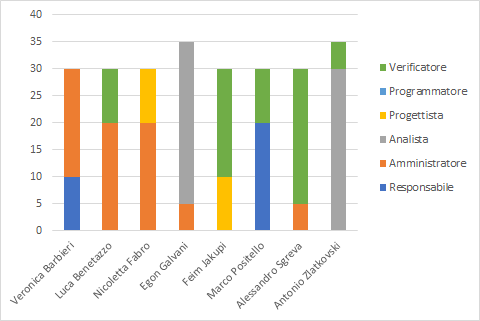
\includegraphics[width=0.7\textwidth]{./res/img/analisi_po.png}
			\caption{Suddivisione oraria del periodo di Analisi}
		\end{figure}

	\newpage
	\subsubsection{Prospetto economico}
		Totale delle ore e costo per ciascun ruolo nel periodo di Analisi:

		\rowcolors{2}{lightRowColor}{darkRowColor}
		\begin{longtable}{
			>{\centering}p{0.25\textwidth}
			>{\centering}p{0.05\textwidth}
			>{\centering\arraybackslash}p{0.15\textwidth} }

			\coloredTableHead
			\textbf{\color{white}Ruolo} &
			\textbf{\color{white}Ore} &
			\textbf{\color{white}Costo in \euro{}}
			\tabularnewline
			\endhead

			% Contenuto della tabella
			% Ruolo & Ore & Costo\\
			Responsabile    & 30  & 900,00 \\
			Amministratore  & 70  & 1.400,00 \\
			Analista        & 60  & 1.500,00 \\
			Progettista     & 20  & 440,00 \\
			Programmatore   & -   & - \\
			Verificatore    & 70  & 1.050,00 \\
			\textbf{Totale} & 250 & 5.290,00 \\

			\rowcolor{white}\caption{Prospetto dei costi per il periodo di Analisi}	\\

		\end{longtable}

		% Grafico
		Rappresentazione grafica della distribuzione dei ruoli:
		\begin{figure}[h]
			\centering
			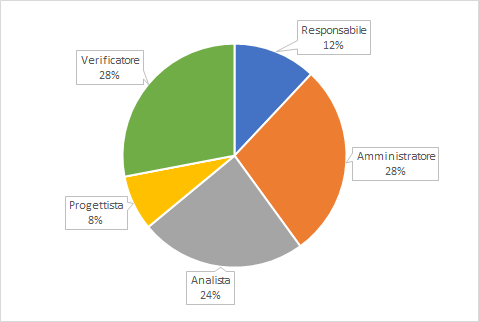
\includegraphics[width=0.7\textwidth]{./res/img/analisi_pe.png}
			\caption{Suddivisione dei ruoli nel periodo di Analisi}
		\end{figure}

\newpage
\subsection{Consolidamento dei Requisiti}
	\subsubsection{Prospetto orario}
		Distribuzione delle ore per ciascun ruolo nel periodo di Consolidamento dei requisiti:

		\rowcolors{2}{lightRowColor}{darkRowColor}
		\begin{longtable}{
			>{\centering}p{0.25\textwidth}
			>{\centering}p{0.05\textwidth}
			>{\centering}p{0.05\textwidth}
			>{\centering}p{0.05\textwidth}
			>{\centering}p{0.05\textwidth}
			>{\centering}p{0.05\textwidth}
			>{\centering}p{0.05\textwidth}
			>{\centering\arraybackslash}p{0.15\textwidth} }

			\coloredTableHead
			\textbf{\color{white}Nome} &
			\textbf{\color{white}Rp} &
			\textbf{\color{white}As} &
			\textbf{\color{white}An} &
			\textbf{\color{white}Pt} &
			\textbf{\color{white}Pr} &
			\textbf{\color{white}Vf} &
			\textbf{\color{white}Totale}
			\tabularnewline
			\endhead

			% Contenuto della tabella
			% Nome & Rp & As & An & Pt & Pr & Vf & Totale \\
			\VB & - & - & 3 & - & - & 2 & 5 \\
			\LB & 5 & - & - & - & - & - & 5 \\
			\NF & - & - & - & - & - & 5 & 5 \\
			\EG & - & 3 & - & - & - & - & 3 \\
			\FJ & - & - & 3 & - & - & 2 & 5 \\
			\MP & - & - & 2 & - & - & 3 & 5 \\
			\AS & - & - & 2 & - & - & 3 & 5 \\
			\AZ & - & 3 & - & - & - & - & 3 \\
			\textbf{Ore totali per ruolo} & 5 & 6 & 10 & - & - & 15 & 36 \\

			\rowcolor{white}\caption {Suddivisione oraria del periodo di Consolidamento dei requisiti} \\

		\end{longtable}

		% Grafico
		Rappresentazione grafica della suddivisione oraria:
		\begin{figure}[h]
			\centering
			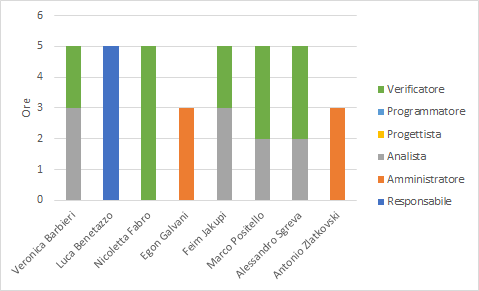
\includegraphics[width=0.7\textwidth]{./res/img/consolidamentoRequisiti_po.png}
			\caption{Suddivisione oraria del periodo di Consolidamento dei requisiti}
		\end{figure}

	\newpage
	\subsubsection{Prospetto economico}
		Totale delle ore e costo per ciascun ruolo nel periodo di Consolidamento dei requisiti:

		\rowcolors{2}{lightRowColor}{darkRowColor}
		\begin{longtable}{
			>{\centering}p{0.25\textwidth}
			>{\centering}p{0.05\textwidth}
			>{\centering\arraybackslash}p{0.15\textwidth} }

			\coloredTableHead
			\textbf{\color{white}Ruolo} &
			\textbf{\color{white}Ore} &
			\textbf{\color{white}Costo in \euro{}}
			\tabularnewline
			\endhead

			% Contenuto della tabella
			% Ruolo & Ore & Costo \\
			Responsabile    & 5  & 150,00 \\
			Amministratore  & 6  & 120,00 \\
			Analista        & 10 & 250,00 \\
			Progettista     & -  & - \\
			Programmatore   & -  & - \\
			Verificatore    & 15 & 225,00 \\
			\textbf{Totale} & 36 & 745,00 \\

			\rowcolor{white}\caption {Prospetto dei costi per il periodo di Consolidamento dei requisiti}	\\

		\end{longtable}

		% Grafico
		Rappresentazione grafica della distribuzione dei ruoli:
		\begin{figure}[h]
			\centering
			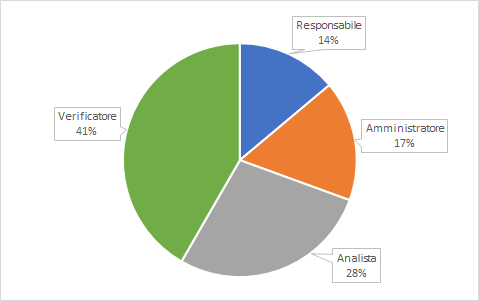
\includegraphics[width=0.7\textwidth]{./res/img/consolidamentoRequisiti_pe.png}
			\caption{Suddivisione dei ruoli nel periodo di Consolidamento dei requisiti}
		\end{figure}

\newpage
\subsection{Progettazione Architetturale}
	\subsubsection{1$^{\circ}$ Incremento}
		\subsubsubsection{Prospetto orario}
		Durante il 1$^{\circ}$ Incremento la distribuzione oraria preventivata dei ruoli di ogni componente del gruppo sarà la seguente:
		\rowcolors{2}{lightRowColor}{darkRowColor}
		\begin{longtable}{
				>{\centering}p{0.25\textwidth}
				>{\centering}p{0.05\textwidth}
				>{\centering}p{0.05\textwidth}
				>{\centering}p{0.05\textwidth}
				>{\centering}p{0.05\textwidth}
				>{\centering}p{0.05\textwidth}
				>{\centering}p{0.05\textwidth}
				>{\centering\arraybackslash}p{0.15\textwidth} }
			
			\coloredTableHead
			\textbf{\color{white}Nome} &
			\textbf{\color{white}Rp} &
			\textbf{\color{white}As} &
			\textbf{\color{white}An} &
			\textbf{\color{white}Pt} &
			\textbf{\color{white}Pr} &
			\textbf{\color{white}Vf} &
			\textbf{\color{white}Totale}
			\tabularnewline
			\endhead
			
			% Contenuto della tabella
			%    Rp & As  An  Pt  Pr  Vf & Totale \\
			\VB & - & -  & - & 2 & - & 2 & 4 \\
			\LB & 2 & -  & - & 2 & - & - & 4 \\
			\NF & - & -  & - & - & - & 4 & 4 \\
			\EG & - & -  & 5 & - & - & - & 5 \\
			\FJ & - & 1  & - & 2 & - & 1 & 4 \\
			\MP & - & 2  & - & 1 & - & 2 & 5 \\
			\AS & - & 2  & - & - & - & 2 & 4 \\
			\AZ & - & -  & 6 & - & - & - & 6 \\
			\textbf{Ore totali per ruolo} & 2 & 5 & 11 & 7 & 0 & 11 & 36 \\
			
			\rowcolor{white}\caption {Suddivisione oraria del primo Incremento} \\
			
		\end{longtable}
		
		% Grafico
		\begin{figure}[H]
			\centering
			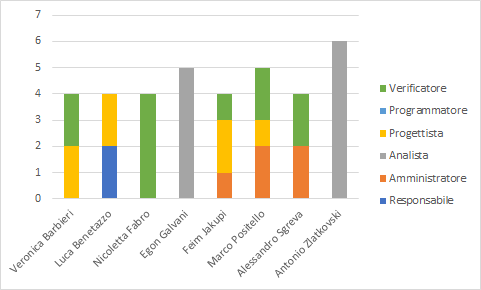
\includegraphics[width=0.7\textwidth]{./res/img/preventivi/inc1_po.png}
			\caption{Suddivisione oraria del primo Incremento}
		\end{figure}
	
		\subsubsubsection{Prospetto economico}
		In base al prospetto orario, quello economico sarà il seguente: 
		\rowcolors{2}{lightRowColor}{darkRowColor}
		\begin{longtable}{
				>{\centering}p{0.25\textwidth}
				>{\centering}p{0.05\textwidth}
				>{\centering\arraybackslash}p{0.15\textwidth} }
			
			\coloredTableHead
			\textbf{\color{white}Ruolo} &
			\textbf{\color{white}Ore} &
			\textbf{\color{white}Costo in \euro{}}
			\tabularnewline
			\endhead
			
			% Contenuto della tabella
			% Ruolo & Ore & Costo \\
			Responsabile    & 2  & 60,00 \\
			Amministratore  & 5  & 100,00 \\
			Analista        & 11  & 275,00 \\
			Progettista     & 7  & 154,00 \\
			Programmatore   & 0  & 0,00 \\
			Verificatore    & 11  & 165,00 \\
			\textbf{Totale} & 36 & 754,00 \\
			
			\rowcolor{white}\caption {Prospetto dei costi per il 1$^{\circ}$ Incremento}	\\
			
		\end{longtable}
		
		% Grafico
		Rappresentazione grafica della distribuzione dei ruoli:
		\begin{figure}[H]
			\centering
			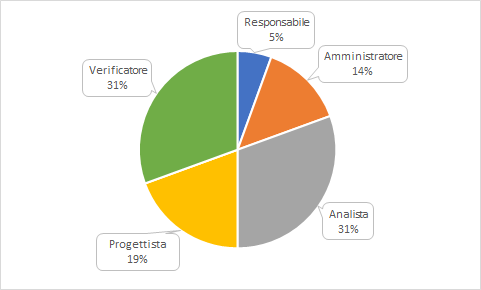
\includegraphics[width=0.7\textwidth]{./res/img/preventivi/inc1_pe.png}
			\caption{Prospetto economico del 1$^{\circ}$ Incremento}
		\end{figure}
	\subsubsection{2$^{\circ}$ Incremento}
		\subsubsubsection{Prospetto orario}
		Durante il 2$^{\circ}$ incremento la distribuzione oraria preventivata dei ruoli di ogni componente del gruppo sarà la seguente:
		\rowcolors{2}{lightRowColor}{darkRowColor}
		\begin{longtable}{
				>{\centering}p{0.25\textwidth}
				>{\centering}p{0.05\textwidth}
				>{\centering}p{0.05\textwidth}
				>{\centering}p{0.05\textwidth}
				>{\centering}p{0.05\textwidth}
				>{\centering}p{0.05\textwidth}
				>{\centering}p{0.05\textwidth}
				>{\centering\arraybackslash}p{0.15\textwidth} }
			
			\coloredTableHead
			\textbf{\color{white}Nome} &
			\textbf{\color{white}Rp} &
			\textbf{\color{white}As} &
			\textbf{\color{white}An} &
			\textbf{\color{white}Pt} &
			\textbf{\color{white}Pr} &
			\textbf{\color{white}Vf} &
			\textbf{\color{white}Totale}
			\tabularnewline
			\endhead
			
			% Contenuto della tabella
			%    Rp & As & An & Pt & Pr & Vf & Totale \\
			\VB & - & -  & - & 2 & 3 & - & 5 \\
			\LB & 1 & -  & 2 & - & 3 & - & 6 \\
			\NF & - & -  & - & - & - & 4 & 4 \\
			\EG & - & -  & 2 & - & - & 2 & 4 \\
			\FJ & - & 1  & - & 2 & 3 & - & 6 \\
			\MP & - & 2  & - & 4 & - & - & 6 \\
			\AS & - & 2  & - & 4 & - & - & 6 \\
			\AZ & - & -  & 4 & - & - & 2 & 6 \\
			\textbf{Ore totali per ruolo} & 1 & 5 & 8 & 12 & 9 & 8 & 43 \\
			
			\rowcolor{white}\caption {Suddivisione oraria del 2$^{\circ}$ incremento} \\
			
		\end{longtable}
		
		% Grafico
		\begin{figure}[H]
			\centering
			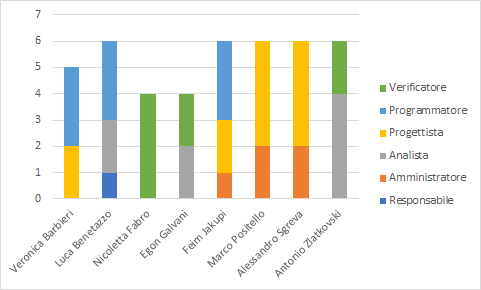
\includegraphics[width=0.7\textwidth]{./res/img/preventivi/inc2_po.png}
			\caption{Suddivisione oraria del 2$^{\circ}$ incremento}
		\end{figure}
	
		\subsubsubsection{Prospetto economico}
		In base al prospetto orario, quello economico sarà il seguente: 
		\rowcolors{2}{lightRowColor}{darkRowColor}
		\begin{longtable}{
				>{\centering}p{0.25\textwidth}
				>{\centering}p{0.05\textwidth}
				>{\centering\arraybackslash}p{0.15\textwidth} }
			
			\coloredTableHead
			\textbf{\color{white}Ruolo} &
			\textbf{\color{white}Ore} &
			\textbf{\color{white}Costo in \euro{}}
			\tabularnewline
			\endhead
			
			% Contenuto della tabella
			% Ruolo & Ore & Costo \\
			Responsabile    & 1  & 30,00 \\
			Amministratore  & 5  & 100,00 \\
			Analista        & 8  & 200,00 \\
			Progettista     & 12  & 264,00 \\
			Programmatore   & 9  & 135,00 \\
			Verificatore    & 8  & 120,00 \\
			\textbf{Totale} & 43 & 849,00 \\
			
			\rowcolor{white}\caption {Prospetto dei costi per il secondo incremento}	\\
			
		\end{longtable}
		
		% Grafico
		Rappresentazione grafica della distribuzione dei ruoli:
		\begin{figure}[H]
			\centering
			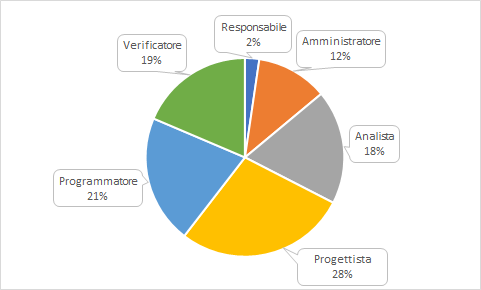
\includegraphics[width=0.7\textwidth]{./res/img/preventivi/inc2_pe.png}
			\caption{Prospetto economico del 2$^{\circ}$ incremento}
		\end{figure}
	\subsubsection{3$^{\circ}$ Incremento}
		\subsubsubsection{Prospetto orario}
		Durante il primo incremento la distribuzione oraria preventivata dei ruoli di ogni componente del gruppo sarà la seguente:
		\rowcolors{2}{lightRowColor}{darkRowColor}
		\begin{longtable}{
				>{\centering}p{0.25\textwidth}
				>{\centering}p{0.05\textwidth}
				>{\centering}p{0.05\textwidth}
				>{\centering}p{0.05\textwidth}
				>{\centering}p{0.05\textwidth}
				>{\centering}p{0.05\textwidth}
				>{\centering}p{0.05\textwidth}
				>{\centering\arraybackslash}p{0.15\textwidth} }
			
			\coloredTableHead
			\textbf{\color{white}Nome} &
			\textbf{\color{white}Rp} &
			\textbf{\color{white}As} &
			\textbf{\color{white}An} &
			\textbf{\color{white}Pt} &
			\textbf{\color{white}Pr} &
			\textbf{\color{white}Vf} &
			\textbf{\color{white}Totale}
			\tabularnewline
			\endhead
			
			% Contenuto della tabella
			%    Rp & As & An & Pt & Pr & Vf & Totale \\
			\VB & - & -  & - & - & 4 & - & 4 \\
			\LB & 1 & -  & 3 & - & 2 & - & 6 \\
			\NF & - & -  & - & 6 & - & - & 6 \\
			\EG & - & -  & - & 2 & - & 4 & 6 \\
			\FJ & - & 1  & - & - & 4 & - & 5 \\
			\MP & - & -  & - & 6 & - & - & 6 \\
			\AS & - & 2  & - & - & - & - & 2 \\
			\AZ & - & -  & - & - & - & 4 & 4 \\
			\textbf{Ore totali per ruolo} & 1 & 3 & 3 & 14 & 10 & 8 & 39 \\
			
			\rowcolor{white}\caption {Suddivisione oraria del terzo incremento} \\
			
		\end{longtable}
		
		% Grafico
		\begin{figure}[H]
			\centering
			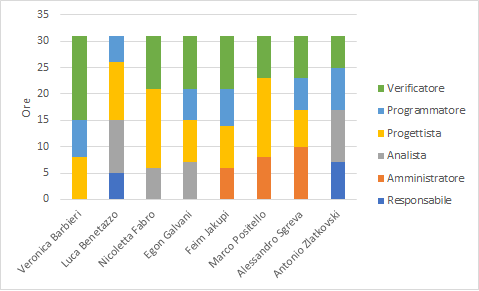
\includegraphics[width=0.7\textwidth]{./res/img/progettazioneArchitetturale_po.png}
			\caption{Suddivisione oraria del terzo incremento}
		\end{figure}
	
		\subsubsubsection{Prospetto economico}
		In base al prospetto orario, quello economico sarà il seguente: 
		\rowcolors{2}{lightRowColor}{darkRowColor}
		\begin{longtable}{
				>{\centering}p{0.25\textwidth}
				>{\centering}p{0.05\textwidth}
				>{\centering\arraybackslash}p{0.15\textwidth} }
			
			\coloredTableHead
			\textbf{\color{white}Ruolo} &
			\textbf{\color{white}Ore} &
			\textbf{\color{white}Costo in \euro{}}
			\tabularnewline
			\endhead
			
			% Contenuto della tabella
			% Ruolo & Ore & Costo \\
			Responsabile    & 1  & 30,00 \\
			Amministratore  & 3  & 60,00 \\
			Analista        & 3  & 75,00 \\
			Progettista     & 14  & 308,00 \\
			Programmatore   & 10 & 150,00 \\
			Verificatore    & 8  & 120,00 \\
			\textbf{Totale} & 39 & 743,00 \\
			
			\rowcolor{white}\caption {Prospetto dei costi per il terzo incremento}	\\
			
		\end{longtable}
		
		% Grafico
		Rappresentazione grafica della distribuzione dei ruoli:
		\begin{figure}[H]
			\centering
			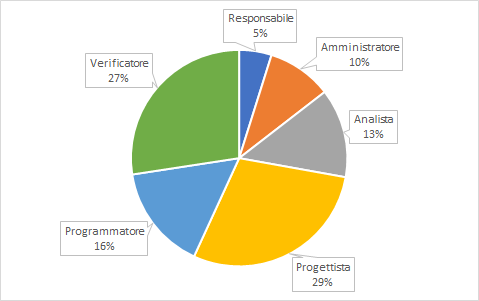
\includegraphics[width=0.7\textwidth]{./res/img/progettazioneArchitetturale_pe.png}
			\caption{Prospetto economico del terzo incremento}
		\end{figure}
	\subsubsection{4$^{\circ}$ Incremento}
		\subsubsubsection{Prospetto orario}
		Durante il quarto incremento la distribuzione oraria preventivata dei ruoli di ogni componente del gruppo sarà la seguente:
		\rowcolors{2}{lightRowColor}{darkRowColor}
		\begin{longtable}{
				>{\centering}p{0.25\textwidth}
				>{\centering}p{0.05\textwidth}
				>{\centering}p{0.05\textwidth}
				>{\centering}p{0.05\textwidth}
				>{\centering}p{0.05\textwidth}
				>{\centering}p{0.05\textwidth}
				>{\centering}p{0.05\textwidth}
				>{\centering\arraybackslash}p{0.15\textwidth} }
			
			\coloredTableHead
			\textbf{\color{white}Nome} &
			\textbf{\color{white}Rp} &
			\textbf{\color{white}As} &
			\textbf{\color{white}An} &
			\textbf{\color{white}Pt} &
			\textbf{\color{white}Pr} &
			\textbf{\color{white}Vf} &
			\textbf{\color{white}Totale}
			\tabularnewline
			\endhead
			
			% Contenuto della tabella
			%    Rp & As & An & Pt & Pr & Vf & Totale \\
			\VB & - & -  & - & - & - & 3 & 3 \\
			\LB & 1 & -  & - & 5 & - & - & 6 \\
			\NF & - & -  & 3 & 3 & - & - & 6 \\
			\EG & - & -  & - & 4 & 2 & - & 6 \\
			\FJ & - & 3  & - & - & - & 1 & 4 \\
			\MP & - & -  & - & 2 & - & 3 & 5 \\
			\AS & - & -  & - & - & 6 & 1 & 7 \\
			\AZ & - & -  & - & - & 2 & - & 2 \\
			\textbf{Ore totali per ruolo} & 1 & 3 & 3 & 14 & 10 & 8 & 39 \\
			
			\rowcolor{white}\caption {Suddivisione oraria del quarto incremento} \\
			
		\end{longtable}
		
		% Grafico
		\begin{figure}[H]
			\centering
			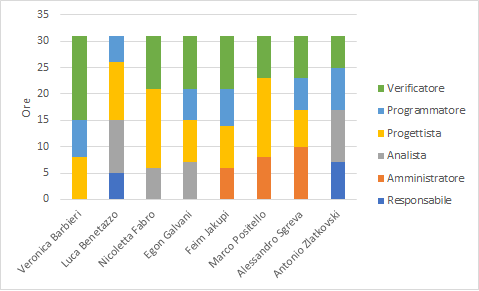
\includegraphics[width=0.7\textwidth]{./res/img/progettazioneArchitetturale_po.png}
			\caption{Suddivisione oraria del quarto incremento}
		\end{figure}
	
		\subsubsubsection{Prospetto economico}
		In base al prospetto orario, quello economico sarà il seguente: 
		\rowcolors{2}{lightRowColor}{darkRowColor}
		\begin{longtable}{
				>{\centering}p{0.25\textwidth}
				>{\centering}p{0.05\textwidth}
				>{\centering\arraybackslash}p{0.15\textwidth} }
			
			\coloredTableHead
			\textbf{\color{white}Ruolo} &
			\textbf{\color{white}Ore} &
			\textbf{\color{white}Costo in \euro{}}
			\tabularnewline
			\endhead
			
			% Contenuto della tabella
			% Ruolo & Ore & Costo \\
			Responsabile    & 1  & 30,00 \\
			Amministratore  & 3  & 60,00 \\
			Analista        & 3  & 75,00 \\
			Progettista     & 14  & 308,00 \\
			Programmatore   & 10 & 150,00 \\
			Verificatore    & 8  & 120,00 \\
			\textbf{Totale} & 39 & 743,00 \\
			
			\rowcolor{white}\caption {Prospetto dei costi per il quarto incremento}	\\
			
		\end{longtable}
		
		% Grafico
		Rappresentazione grafica della distribuzione dei ruoli:
		\begin{figure}[H]
			\centering
			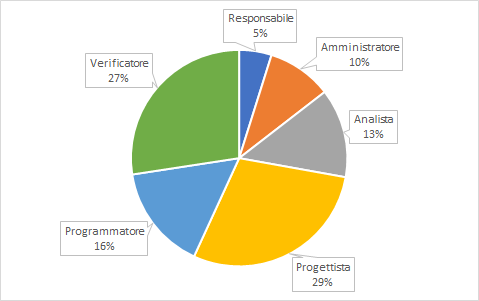
\includegraphics[width=0.7\textwidth]{./res/img/progettazioneArchitetturale_pe.png}
			\caption{Prospetto economico del quarto incremento}
		\end{figure}
	\subsubsection{5$^{\circ}$ Incremento}
		\subsubsubsection{Prospetto orario}
		Durante il 5$^{\circ}$ incremento la distribuzione oraria preventivata dei ruoli di ogni componente del gruppo sarà la seguente:
		\rowcolors{2}{lightRowColor}{darkRowColor}
		\begin{longtable}{
				>{\centering}p{0.25\textwidth}
				>{\centering}p{0.05\textwidth}
				>{\centering}p{0.05\textwidth}
				>{\centering}p{0.05\textwidth}
				>{\centering}p{0.05\textwidth}
				>{\centering}p{0.05\textwidth}
				>{\centering}p{0.05\textwidth}
				>{\centering\arraybackslash}p{0.15\textwidth} }
			
			\coloredTableHead
			\textbf{\color{white}Nome} &
			\textbf{\color{white}Rp} &
			\textbf{\color{white}As} &
			\textbf{\color{white}An} &
			\textbf{\color{white}Pt} &
			\textbf{\color{white}Pr} &
			\textbf{\color{white}Vf} &
			\textbf{\color{white}Totale}
			\tabularnewline
			\endhead
			
			% Contenuto della tabella
			%    Rp & As & An & Pt & Pr & Vf & Totale \\
			\VB & - & - & - & - & - & 4 & 4 \\
			\LB & - & - & 3 & - & - & - & 3 \\
			\NF & - & - & - & 3 & - & - & 3 \\
			\EG & - & - & - & 2 & 4 & - & 6 \\
			\FJ & - & - & - & 4 & - & - & 4 \\
			\MP & - & - & - & 2 & - & 3 & 5 \\
			\AS & - & 3 & - & 1 & - & - & 4 \\
			\AZ & 2 & - & - & - & 6 & - & 8 \\
			\textbf{Ore totali per ruolo} & 2 & 3 & 3 & 12 & 10 & 7 & 37 \\
			
			\rowcolor{white}\caption {Suddivisione oraria del 5$^{\circ}$ incremento} \\
			
		\end{longtable}
		
		% Grafico
		\begin{figure}[H]
			\centering
			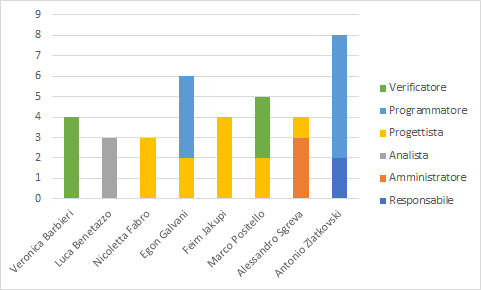
\includegraphics[width=0.7\textwidth]{./res/img/preventivi/inc5_po.png}
			\caption{Suddivisione oraria del 5$^{\circ}$ incremento}
		\end{figure}
	
		\subsubsubsection{Prospetto economico}
		In base al prospetto orario, quello economico sarà il seguente: 
		\rowcolors{2}{lightRowColor}{darkRowColor}
		\begin{longtable}{
				>{\centering}p{0.25\textwidth}
				>{\centering}p{0.05\textwidth}
				>{\centering\arraybackslash}p{0.15\textwidth} }
			
			\coloredTableHead
			\textbf{\color{white}Ruolo} &
			\textbf{\color{white}Ore} &
			\textbf{\color{white}Costo in \euro{}}
			\tabularnewline
			\endhead
			
			% Contenuto della tabella
			% Ruolo & Ore & Costo \\
			Responsabile    & 2  & 60,00 \\
			Amministratore  & 3  & 60,00 \\
			Analista        & 3  & 75,00 \\
			Progettista     & 12  & 264,00 \\
			Programmatore   & 10  & 150,00 \\
			Verificatore    & 7  & 105,00 \\
			\textbf{Totale} & 37 & 714,00 \\
			
			\rowcolor{white}\caption {Prospetto dei costi per il 5$^{\circ}$ incremento}	\\
			
		\end{longtable}
		
		% Grafico
		Rappresentazione grafica della distribuzione dei ruoli:
		\begin{figure}[H]
			\centering
			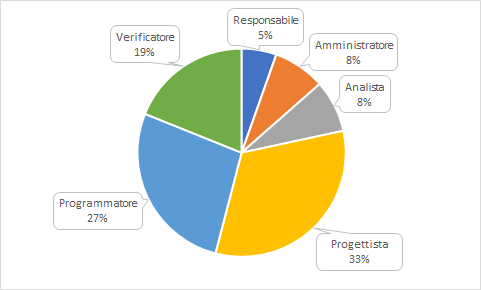
\includegraphics[width=0.7\textwidth]{./res/img/preventivi/inc5_pe.png}
			\caption{Prospetto economico del 5$^{\circ}$ incremento}
		\end{figure}
	\subsubsection{6$^{\circ}$ Incremento}
		\subsubsubsection{Prospetto orario}
		Durante il sesto incremento la distribuzione oraria preventivata dei ruoli di ogni componente del gruppo sarà la seguente:
		\rowcolors{2}{lightRowColor}{darkRowColor}
		\begin{longtable}{
				>{\centering}p{0.25\textwidth}
				>{\centering}p{0.05\textwidth}
				>{\centering}p{0.05\textwidth}
				>{\centering}p{0.05\textwidth}
				>{\centering}p{0.05\textwidth}
				>{\centering}p{0.05\textwidth}
				>{\centering}p{0.05\textwidth}
				>{\centering\arraybackslash}p{0.15\textwidth} }
			
			\coloredTableHead
			\textbf{\color{white}Nome} &
			\textbf{\color{white}Rp} &
			\textbf{\color{white}As} &
			\textbf{\color{white}An} &
			\textbf{\color{white}Pt} &
			\textbf{\color{white}Pr} &
			\textbf{\color{white}Vf} &
			\textbf{\color{white}Totale}
			\tabularnewline
			\endhead
			
			% Contenuto della tabella
			%    Rp & As & An & Pt & Pr & Vf & Totale \\
			\VB & - & -  & - & 2 & - & 2 & 4 \\
			\LB & - & -  & 2 & 2 & - & - & 4 \\
			\NF & - & -  & 2 & 2 & - & 2 & 6 \\
			\EG & - & -  & - & - & - & 2 & 2 \\
			\FJ & - & -  & - & - & - & 4 & 4 \\
			\MP & - & 1  & - & - & - & - & 1 \\
			\AS & - & 2  & - & 1 & - & 3 & 6 \\
			\AZ & 2 & -  & - & - & - & - & 2 \\
			\textbf{Ore totali per ruolo} & 2 & 3 & 4 & 7 & 0 & 13 & 29 \\
			
			\rowcolor{white}\caption {Suddivisione oraria del primo incremento} \\
			
		\end{longtable}
		
		% Grafico
		\begin{figure}[h]
			\centering
			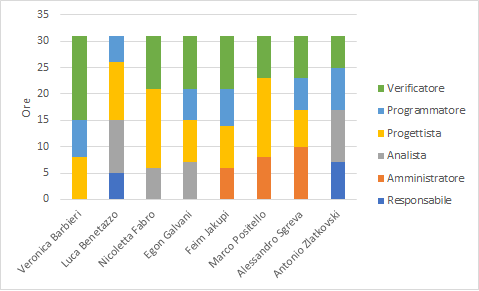
\includegraphics[width=0.7\textwidth]{./res/img/progettazioneArchitetturale_po.png}
			\caption{Suddivisione oraria del sesto incremento}
		\end{figure}
	
		\subsubsubsection{Prospetto economico}
		In base al prospetto orario, quello economico sarà il seguente: 
		\rowcolors{2}{lightRowColor}{darkRowColor}
		\begin{longtable}{
				>{\centering}p{0.25\textwidth}
				>{\centering}p{0.05\textwidth}
				>{\centering\arraybackslash}p{0.15\textwidth} }
			
			\coloredTableHead
			\textbf{\color{white}Ruolo} &
			\textbf{\color{white}Ore} &
			\textbf{\color{white}Costo in \euro{}}
			\tabularnewline
			\endhead
			
			% Contenuto della tabella
			% Ruolo & Ore & Costo \\
			Responsabile    & 2  & 60,00 \\
			Amministratore  & 3  & 60,00 \\
			Analista        & 4  & 100,00 \\
			Progettista     & 7  & 154,00 \\
			Programmatore   & 0  & 0,00 \\
			Verificatore    & 13  & 195,00 \\
			\textbf{Totale} & 29 & 569,00 \\
			
			\rowcolor{white}\caption {Prospetto dei costi per il sesto incremento}	\\
			
		\end{longtable}
		
		% Grafico
		Rappresentazione grafica della distribuzione dei ruoli:
		\begin{figure}[h]
			\centering
			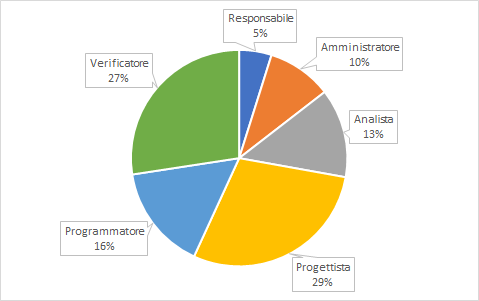
\includegraphics[width=0.7\textwidth]{./res/img/progettazioneArchitetturale_pe.png}
			\caption{Prospetto economico del sesto incremento}
		\end{figure}
	\subsubsection{7$^{\circ}$ Incremento}
		\subsubsubsection{Prospetto orario}
		Durante il 7$^{\circ}$ incremento la distribuzione oraria preventivata dei ruoli di ogni componente del gruppo sarà la seguente:
		\rowcolors{2}{lightRowColor}{darkRowColor}
		\begin{longtable}{
				>{\centering}p{0.25\textwidth}
				>{\centering}p{0.05\textwidth}
				>{\centering}p{0.05\textwidth}
				>{\centering}p{0.05\textwidth}
				>{\centering}p{0.05\textwidth}
				>{\centering}p{0.05\textwidth}
				>{\centering}p{0.05\textwidth}
				>{\centering\arraybackslash}p{0.15\textwidth} }
			
			\coloredTableHead
			\textbf{\color{white}Nome} &
			\textbf{\color{white}Rp} &
			\textbf{\color{white}As} &
			\textbf{\color{white}An} &
			\textbf{\color{white}Pt} &
			\textbf{\color{white}Pr} &
			\textbf{\color{white}Vf} &
			\textbf{\color{white}Totale}
			\tabularnewline
			\endhead
			
			% Contenuto della tabella
			%    Rp & As & An & Pt & Pr & Vf & Totale \\
			\VB & - & -  & - & 2 & - & 4 & 6 \\
			\LB & - & -  & - & 2 & - & - & 2 \\
			\NF & - & -  & 1 & 1 & - & - & 2 \\
			\EG & - & -  & - & - & - & 2 & 2 \\
			\FJ & - & -  & - & - & - & 3 & 3 \\
			\MP & - & 1  & - & - & - & - & 1 \\
			\AS & - & -  & - & 1 & - & 2 & 3 \\
			\AZ & 2 & -  & - & - & - & - & 2 \\
			\textbf{Ore totali per ruolo} & 2 & 1 & 1 & 6 & 0 & 11 & 21 \\
			
			\rowcolor{white}\caption {Suddivisione oraria del 7$^{\circ}$ incremento} \\
			
		\end{longtable}
		
		% Grafico
		\begin{figure}[H]
			\centering
			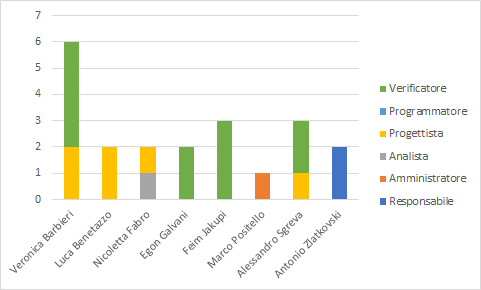
\includegraphics[width=0.7\textwidth]{./res/img/preventivi/inc7_po.png}
			\caption{Suddivisione oraria del 7$^{\circ}$ incremento}
		\end{figure}
	
		\subsubsubsection{Prospetto economico}
		In base al prospetto orario, quello economico sarà il seguente: 
		\rowcolors{2}{lightRowColor}{darkRowColor}
		\begin{longtable}{
				>{\centering}p{0.25\textwidth}
				>{\centering}p{0.05\textwidth}
				>{\centering\arraybackslash}p{0.15\textwidth} }
			
			\coloredTableHead
			\textbf{\color{white}Ruolo} &
			\textbf{\color{white}Ore} &
			\textbf{\color{white}Costo in \euro{}}
			\tabularnewline
			\endhead
			
			% Contenuto della tabella
			% Ruolo & Ore & Costo \\
			Responsabile    & 2  & 60,00 \\
			Amministratore  & 1  & 20,00 \\
			Analista        & 1  & 25,00 \\
			Progettista     & 6  & 132,00 \\
			Programmatore   & 0  & 0,00 \\
			Verificatore    & 11  & 165,00 \\
			\textbf{Totale} & 21 & 402,00 \\
			
			\rowcolor{white}\caption {Prospetto dei costi per il 7$^{\circ}$ incremento}	\\
			
		\end{longtable}
		
		% Grafico
		Rappresentazione grafica della distribuzione dei ruoli:
		\begin{figure}[H]
			\centering
			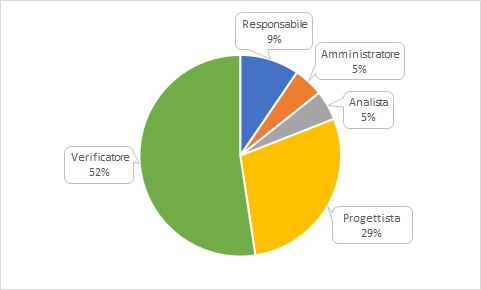
\includegraphics[width=0.7\textwidth]{./res/img/preventivi/inc7_pe.png}
			\caption{Prospetto economico del 7$^{\circ}$ incremento}
		\end{figure}
	\subsubsection{8$^{\circ}$ Incremento}
		\subsubsubsection{Prospetto orario}
		Durante l'8$^{\circ}$ Incremento la distribuzione oraria preventivata dei ruoli di ogni componente del gruppo sarà la seguente:
		\rowcolors{2}{lightRowColor}{darkRowColor}
		\begin{longtable}{
				>{\centering}p{0.25\textwidth}
				>{\centering}p{0.05\textwidth}
				>{\centering}p{0.05\textwidth}
				>{\centering}p{0.05\textwidth}
				>{\centering}p{0.05\textwidth}
				>{\centering}p{0.05\textwidth}
				>{\centering}p{0.05\textwidth}
				>{\centering\arraybackslash}p{0.15\textwidth} }
			
			\coloredTableHead
			\textbf{\color{white}Nome} &
			\textbf{\color{white}Rp} &
			\textbf{\color{white}As} &
			\textbf{\color{white}An} &
			\textbf{\color{white}Pt} &
			\textbf{\color{white}Pr} &
			\textbf{\color{white}Vf} &
			\textbf{\color{white}Totale}
			\tabularnewline
			\endhead
			
			% Contenuto della tabella
			%    Rp & As & An & Pt & Pr & Vf & Totale \\
			\VB & - & -  & - & - & - & 1 & 1 \\
			\LB & - & -  & - & - & - & - & - \\
			\NF & - & -  & - & - & - & - & - \\
			\EG & - & -  & - & - & - & - & - \\
			\FJ & - & -  & - & - & - & 1 & 1 \\
			\MP & - & -  & - & - & - & - & - \\
			\AS & - & 1  & - & - & - & - & 1 \\
			\AZ & 1 & -  & - & - & - & - & 1 \\
			\textbf{Ore totali per ruolo} & 1 & 1 & 0 & 0 & 0 & 2 & 4 \\
			
			\rowcolor{white}\caption {Suddivisione oraria dell'8$^{\circ}$ Incremento} \\
			
		\end{longtable}
		
		% Grafico
		\begin{figure}[H]
			\centering
			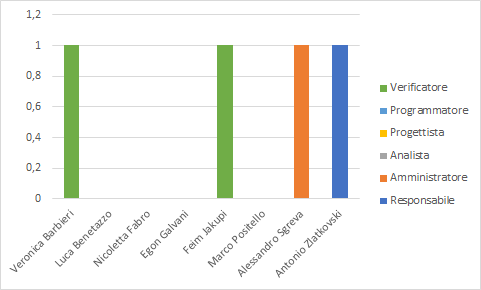
\includegraphics[width=0.7\textwidth]{./res/img/preventivi/inc8_po.png}
			\caption{Suddivisione oraria dell'8$^{\circ}$ Incremento}
		\end{figure}
	
		\subsubsubsection{Prospetto economico}
		In base al prospetto orario, quello economico sarà il seguente: 
		\rowcolors{2}{lightRowColor}{darkRowColor}
		\begin{longtable}{
				>{\centering}p{0.25\textwidth}
				>{\centering}p{0.05\textwidth}
				>{\centering\arraybackslash}p{0.15\textwidth} }
			
			\coloredTableHead
			\textbf{\color{white}Ruolo} &
			\textbf{\color{white}Ore} &
			\textbf{\color{white}Costo in \euro{}}
			\tabularnewline
			\endhead
			
			% Contenuto della tabella
			% Ruolo & Ore & Costo \\
			Responsabile    & 1  & 30,00 \\
			Amministratore  & 1  & 20,00 \\
			Analista        & 0  & 0,00 \\
			Progettista     & 0  & 0,00 \\
			Programmatore   & 0  & 0,00 \\
			Verificatore    & 2  & 30,00 \\
			\textbf{Totale} & 4 & 80,00 \\
			
			\rowcolor{white}\caption {Prospetto dei costi per il periodo dell'8$^{\circ}$ Incremento}	\\
			
		\end{longtable}
		
		% Grafico
		Rappresentazione grafica della distribuzione dei ruoli:
		\begin{figure}[H]
			\centering
			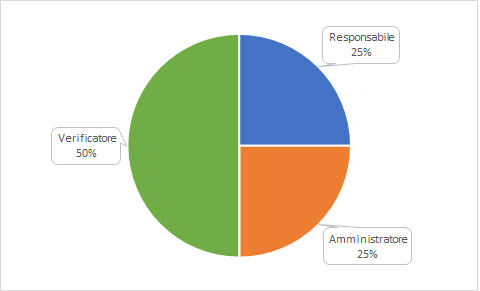
\includegraphics[width=0.7\textwidth]{./res/img/preventivi/inc8_pe.png}
			\caption{Prospetto economico dell'8$^{\circ}$ Incremento}
		\end{figure}
	\subsubsection{Periodo complessivo}

	\subsubsubsection{Prospetto orario}
		Distribuzione delle ore per ciascun ruolo nel periodo di Progettazione Architetturale:

		\rowcolors{2}{lightRowColor}{darkRowColor}
		\begin{longtable}{
			>{\centering}p{0.25\textwidth}
			>{\centering}p{0.05\textwidth}
			>{\centering}p{0.05\textwidth}
			>{\centering}p{0.05\textwidth}
			>{\centering}p{0.05\textwidth}
			>{\centering}p{0.05\textwidth}
			>{\centering}p{0.05\textwidth}
			>{\centering\arraybackslash}p{0.15\textwidth} }

			\coloredTableHead
			\textbf{\color{white}Nome} &
			\textbf{\color{white}Rp} &
			\textbf{\color{white}As} &
			\textbf{\color{white}An} &
			\textbf{\color{white}Pt} &
			\textbf{\color{white}Pr} &
			\textbf{\color{white}Vf} &
			\textbf{\color{white}Totale}
			\tabularnewline
			\endhead

			% Contenuto della tabella
			% Nome & Rp & As & An & Pt & Pr & Vf & Totale \\
			\VB & - & -  & -  & 8  & 7 & 16 & 31 \\
			\LB & 5 & -  & 10 & 11 & 5 & -  & 31 \\
			\NF & - & -  & 6  & 15 & - & 10 & 31 \\
			\EG & - & -  & 7  & 8  & 6 & 10 & 31 \\
			\FJ & - & 6  & -  & 8  & 7 & 10 & 31 \\
			\MP & - & 8  & -  & 15 & - & 8  & 31 \\
			\AS & - & 10 & -  & 7  & 6 & 8  & 31 \\
			\AZ & 7 & -  & 10 & -  & 8 & 6  & 31 \\
			\textbf{Ore totali per ruolo} & 12 & 24 & 33 & 72 & 39 & 68 & 248 \\

			\rowcolor{white}\caption {Suddivisione oraria del periodo di Progettazione Architetturale} \\

		\end{longtable}

		% Grafico
		\begin{figure}[H]
			\centering
			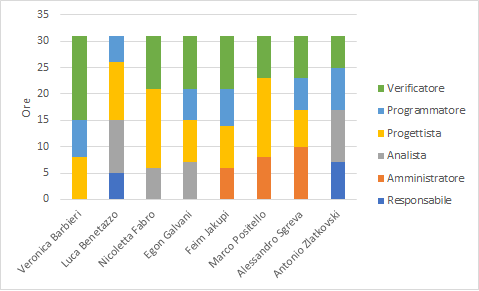
\includegraphics[width=0.7\textwidth]{./res/img/progettazioneArchitetturale_po.png}
			\caption{Suddivisione oraria del periodo di Progettazione Architetturale}
		\end{figure}

	\subsubsubsection{Prospetto economico}
		Totale delle ore e costo per ciascun ruolo nel periodo di Progettazione Architetturale:

		\rowcolors{2}{lightRowColor}{darkRowColor}
		\begin{longtable}{
			>{\centering}p{0.25\textwidth}
			>{\centering}p{0.05\textwidth}
			>{\centering\arraybackslash}p{0.15\textwidth} }

			\coloredTableHead
			\textbf{\color{white}Ruolo} &
			\textbf{\color{white}Ore} &
			\textbf{\color{white}Costo in \euro{}}
			\tabularnewline
			\endhead

			% Contenuto della tabella
			% Ruolo & Ore & Costo \\
			Responsabile    & 12  & 360,00 \\
			Amministratore  & 24  & 480,00 \\
			Analista        & 33  & 825,00 \\
			Progettista     & 72  & 1.584,00 \\
			Programmatore   & 39  & 585,00 \\
			Verificatore    & 68  & 1.020,00 \\
			\textbf{Totale} & 248 & 4.854,00 \\

			\rowcolor{white}\caption {Prospetto dei costi per il periodo di Progettazione Architetturale}	\\

		\end{longtable}

		% Grafico
		Rappresentazione grafica della distribuzione dei ruoli:
		\begin{figure}[H]
			\centering
			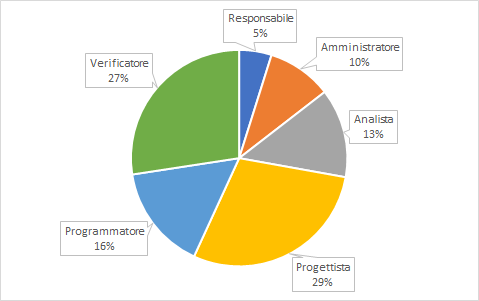
\includegraphics[width=0.7\textwidth]{./res/img/progettazioneArchitetturale_pe.png}
			\caption{Suddivisione dei ruoli nel periodo di Progettazione Architetturale}
		\end{figure}

	
\newpage	
\subsection{Progettazione di Dettaglio e Codifica}
	\subsubsection{9$^{\circ}$ Incremento}
		\subsubsubsection{Prospetto orario}
		Durante il 9$^{\circ}$ Incremento la distribuzione oraria preventivata dei ruoli di ogni componente del gruppo sarà la seguente:
		\rowcolors{2}{lightRowColor}{darkRowColor}
		\begin{longtable}{
				>{\centering}p{0.25\textwidth}
				>{\centering}p{0.05\textwidth}
				>{\centering}p{0.05\textwidth}
				>{\centering}p{0.05\textwidth}
				>{\centering}p{0.05\textwidth}
				>{\centering}p{0.05\textwidth}
				>{\centering}p{0.05\textwidth}
				>{\centering\arraybackslash}p{0.15\textwidth} }
			
			\coloredTableHead
			\textbf{\color{white}Nome} &
			\textbf{\color{white}Rp} &
			\textbf{\color{white}As} &
			\textbf{\color{white}An} &
			\textbf{\color{white}Pt} &
			\textbf{\color{white}Pr} &
			\textbf{\color{white}Vf} &
			\textbf{\color{white}Totale}
			\tabularnewline
			\endhead
			
			% Contenuto della tabella
			%    Rp & As & An & Pt & Pr & Vf & Totale \\
			\VB & - & 2  & - & - & - & 4 & 6 \\
			\LB & - & -  & - & 4 & - & - & 4 \\
			\NF & - & 4  & - & - & - & - & 4 \\
			\EG & 2 & -  & - & 2 & - & - & 4 \\
			\FJ & - & -  & - & - & - & 4 & 4 \\
			\MP & - & -  & - & 2 & - & 3 & 5 \\
			\AS & - & -  & - & 2 & - & 2 & 4 \\
			\AZ & - & 2  & - & - & - & 2 & 4 \\
			\textbf{Ore totali per ruolo} & 2 & 8 & 0 & 10 & 0 & 15 & 35 \\
			
			\rowcolor{white}\caption {Suddivisione oraria del 9$^{\circ}$ Incremento} \\
			
		\end{longtable}
		
		% Grafico
		\begin{figure}[H]
			\centering
			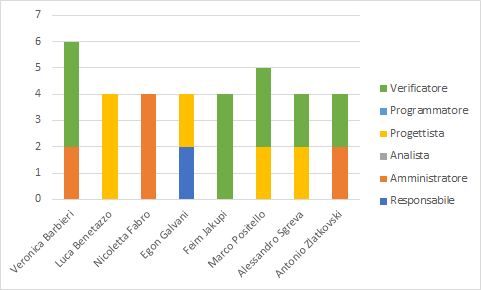
\includegraphics[width=0.7\textwidth]{./res/img/preventivi/inc9_po.png}
			\caption{Suddivisione oraria del 9$^{\circ}$ Incremento}
		\end{figure}
	
		\subsubsubsection{Prospetto economico}
		In base al prospetto orario, quello economico sarà il seguente: 
		\rowcolors{2}{lightRowColor}{darkRowColor}
		\begin{longtable}{
				>{\centering}p{0.25\textwidth}
				>{\centering}p{0.05\textwidth}
				>{\centering\arraybackslash}p{0.15\textwidth} }
			
			\coloredTableHead
			\textbf{\color{white}Ruolo} &
			\textbf{\color{white}Ore} &
			\textbf{\color{white}Costo in \euro{}}
			\tabularnewline
			\endhead
			
			% Contenuto della tabella
			% Ruolo & Ore & Costo \\
			Responsabile    & 2  & 60,00 \\
			Amministratore  & 8  & 160,00 \\
			Analista        & 0  & 0,00 \\
			Progettista     & 10  & 220,00 \\
			Programmatore   & 0  & 0,00 \\
			Verificatore    & 15  & 225,00 \\
			\textbf{Totale} & 35 & 665,00 \\
			
			\rowcolor{white}\caption {Prospetto dei costi per il 9$^{\circ}$ Incremento}	\\
			
		\end{longtable}
		
		% Grafico
		Rappresentazione grafica della distribuzione dei ruoli:
		\begin{figure}[H]
			\centering
			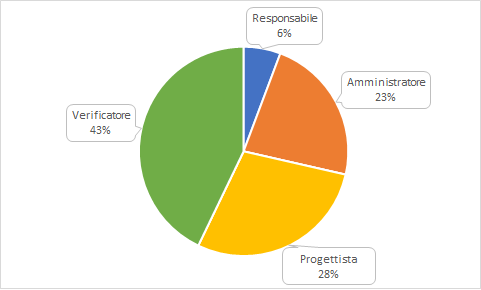
\includegraphics[width=0.7\textwidth]{./res/img/preventivi/inc9_pe.png}
			\caption{Prospetto economico del 9$^{\circ}$ Incremento}
		\end{figure}
	\subsubsection{10$^{\circ}$ Incremento}
	
	\subsubsubsection{Consuntivo}
					
		\begin{longtable}{
				>{\centering}p{0.25\textwidth}
				>{\centering}p{0.08\textwidth}
				>{\centering}p{0.08\textwidth}
				>{\centering}p{0.15\textwidth}
				>{\centering\arraybackslash}p{0.15\textwidth} }
			
			\coloredTableHead
			\textbf{\color{white}Ruolo} &
			\textbf{\color{white}Ore} &
			\textbf{\color{white}Delta ore} &
			\textbf{\color{white}Costo in \euro{}} &
			\textbf{\color{white}Delta costo}
			\tabularnewline
			\endhead
			
			% Contenuto della tabella
			% Ruolo & OreEffettive & DeltaOre & Costo & DeltaCosto \\
			Responsabile    & 4 & +0 &   120,00 & +  0,00 \\
			Amministratore  & 4 & +0 &   80,00 & +  0,00 \\
			Analista        & 0 & +0 &   0,00 & + 0,00 \\
			Progettista     & 39 & +4 & 858,00 & + 88,00 \\
			Programmatore   & 23 & -2 &  345,00 & - 30,00 \\
			Verificatore    & 25 & +0 & 375,00 & + 0,00 \\
			\textbf{Totale Effettivo} & \multicolumn{2}{c}{\textbf{95}} & \multicolumn{2}{c}{\textbf{1778,00}} \\
			\textbf{Delta} & \multicolumn{2}{c}{\textbf{+2}} & \multicolumn{2}{c}{\textbf{+58,00}} \\
			
			\rowcolor{white}\caption{Consuntivo per il 10$^{\circ}$ Incremento}	\\
			
		\end{longtable}
		
	\subsubsubsection{Conclusioni}
	In questo periodo il gruppo si è impegnato nella progettazione e scelta dell'architettura da applicare al prodotto\ped{\textit{G}}. Tale procedimento ha richiesto più tempo del previsto, portando alla necessità di un numero di ore superiore a quanto pianificato per il ruolo di Progettista. \\
	L'attività di codifica è stata leggermente meno dispendiosa del previsto, a causa dell'utilizzo del prototipo ottenuto dalla fase precedente. 
	
	\subsubsubsection{Preventivo a finire rispetto al periodo}
	Il bilancio è \textbf{negativo}, con una spesa in eccesso di \textbf{58,00\euro{}}. Non si ritiene necessaria alcuna ripianificazione, poichè la somma non è significativa. 
	Il soddisfacimento degli obiettivi pianificati ha richiesto un quantitativo di ore superiore a quanto previsto, che hanno portato a questo bilancio negativo.
	
	\subsubsubsection{Preventivo a finire complessivo}	
	Date le considerazioni precedenti su costi e obiettivi, il preventivo complessivo resta invariato.
	\subsubsection{11$^{\circ}$ Incremento}
	
	\subsubsubsection{Consuntivo}
		\begin{longtable}{
				>{\centering}p{0.25\textwidth}
				>{\centering}p{0.08\textwidth}
				>{\centering}p{0.08\textwidth}
				>{\centering}p{0.15\textwidth}
				>{\centering\arraybackslash}p{0.15\textwidth} }
			
			\coloredTableHead
			\textbf{\color{white}Ruolo} &
			\textbf{\color{white}Ore} &
			\textbf{\color{white}Delta ore} &
			\textbf{\color{white}Costo in \euro{}} &
			\textbf{\color{white}Delta costo}
			\tabularnewline
			\endhead
			
			% Contenuto della tabella
			% Ruolo & OreEffettive & DeltaOre & Costo & DeltaCosto \\
			Responsabile    & 3 & +0 &   90,00 & +  0,00 \\
			Amministratore  & 4 & +0 &   80,00 & +  0,00 \\
			Analista        & 0 & +0 &   0,00 & + 0,00 \\
			Progettista     & 10 & +0 & 220,00 & + 0,00 \\
			Programmatore   & 35 & -7 &   525,00 &  -105,00 \\
			Verificatore    & 15 & +0 & 225,00 & + 0,00 \\
			\textbf{Totale Effettivo} & \multicolumn{2}{c}{\textbf{64}} & \multicolumn{2}{c}{\textbf{1140,00}} \\
			\textbf{Delta} & \multicolumn{2}{c}{\textbf{-10}} & \multicolumn{2}{c}{\textbf{-105,00}} \\
			
			\rowcolor{white}\caption{Consuntivo per l'11$^{\circ}$ Incremento}	\\
			
		\end{longtable}
		
	\subsubsubsection{Conclusioni}
	In questo periodo il gruppo si è impegnato principalmente nell'adattare la struttura del prototipo ottenuto dalla fase precedente alla progettazione identificata nell'Incremento 10. Tale attività ha richiesto un notevole numero di ore di codifica in meno rispetto a quanto previsto, poichè la struttura del prototipo seguiva già in parte quella decisa durante la progettazione. 
	
	\subsubsubsection{Preventivo a finire rispetto al periodo}
	Il bilancio è \textbf{positivo}, con un risparmio di \textbf{105,00\euro{}}.  Tale somma
	andrà a bilanciare il leggero deficit ottenuto nell'Incremento precedente. La differenza
	rispetto ai costi preventivati fino a questo punto sarà quindi poco consistente, perciò non si
	reputa necessaria una ripianificazione delle attività di progetto.
	
	\subsubsubsection{Preventivo a finire complessivo}	
	Date le considerazioni precedenti, il preventivo complessivo resta invariato.
	\subsubsection{12$^{\circ}$ Incremento}
		\subsubsubsection{Prospetto orario}
		Durante il 12$^{\circ}$ incremento la distribuzione oraria preventivata dei ruoli di ogni componente del gruppo sarà la seguente:
		\rowcolors{2}{lightRowColor}{darkRowColor}
		\begin{longtable}{
				>{\centering}p{0.25\textwidth}
				>{\centering}p{0.05\textwidth}
				>{\centering}p{0.05\textwidth}
				>{\centering}p{0.05\textwidth}
				>{\centering}p{0.05\textwidth}
				>{\centering}p{0.05\textwidth}
				>{\centering}p{0.05\textwidth}
				>{\centering\arraybackslash}p{0.15\textwidth} }
			
			\coloredTableHead
			\textbf{\color{white}Nome} &
			\textbf{\color{white}Rp} &
			\textbf{\color{white}As} &
			\textbf{\color{white}An} &
			\textbf{\color{white}Pt} &
			\textbf{\color{white}Pr} &
			\textbf{\color{white}Vf} &
			\textbf{\color{white}Totale}
			\tabularnewline
			\endhead
			
			% Contenuto della tabella
			%    Rp & As & An & Pt & Pr & Vf & Totale \\
			\VB & - & -  & - & - & 10 & - & 10 \\
			\LB & - & -  & - & 4 & 10 & - & 14 \\
			\NF & - & -  & - & - & 10 & - & 10 \\
			\EG & - & -  & - & - & 10 & 2 & 12 \\
			\FJ & 2 & -  & - & 4 & - & 1 & 7 \\
			\MP & 1 & -  & - & - & 5 & 2 & 8 \\
			\AS & - & -  & - & 2 & - & 5 & 7 \\
			\AZ & - & 3  & - & - & - & 5 & 8 \\
			\textbf{Ore totali per ruolo} & 3 & 3 & 0 & 10 & 45 & 15 & 76 \\
			
			\rowcolor{white}\caption {Suddivisione oraria del 12$^{\circ}$ incremento} \\
			
		\end{longtable}
		
		% Grafico
		\begin{figure}[H]
			\centering
			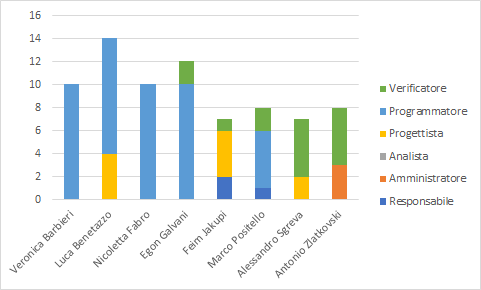
\includegraphics[width=0.7\textwidth]{./res/img/preventivi/inc12_po.png}
			\caption{Suddivisione oraria del 12$^{\circ}$ incremento}
		\end{figure}
	
		\subsubsubsection{Prospetto economico}
		In base al prospetto orario, quello economico sarà il seguente: 
		\rowcolors{2}{lightRowColor}{darkRowColor}
		\begin{longtable}{
				>{\centering}p{0.25\textwidth}
				>{\centering}p{0.05\textwidth}
				>{\centering\arraybackslash}p{0.15\textwidth} }
			
			\coloredTableHead
			\textbf{\color{white}Ruolo} &
			\textbf{\color{white}Ore} &
			\textbf{\color{white}Costo in \euro{}}
			\tabularnewline
			\endhead
			
			% Contenuto della tabella
			% Ruolo & Ore & Costo \\
			Responsabile    & 3  & 90,00 \\
			Amministratore  & 3  & 60,00 \\
			Analista        & 0  & 0,00 \\
			Progettista     & 10  & 220,00 \\
			Programmatore   & 45 & 675,00 \\
			Verificatore    & 15  & 225,00 \\
			\textbf{Totale} & 76 & 1270,00 \\
			
			\rowcolor{white}\caption {Prospetto dei costi per il 12$^{\circ}$ incremento}	\\
			
		\end{longtable}
		
		% Grafico
		Rappresentazione grafica della distribuzione dei ruoli:
		\begin{figure}[H]
			\centering
			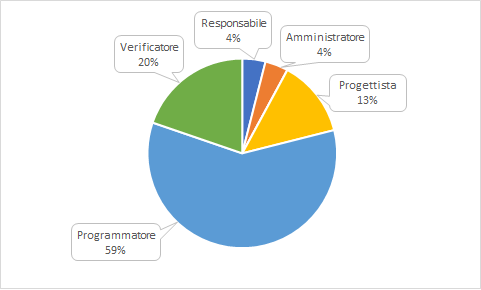
\includegraphics[width=0.7\textwidth]{./res/img/preventivi/inc12_pe.png}
			\caption{Prospetto economico del 12$^{\circ}$ incremento}
		\end{figure}
	\subsubsection{13$^{\circ}$ Incremento}
	
	\subsubsubsection{Consuntivo}
		\begin{longtable}{
				>{\centering}p{0.25\textwidth}
				>{\centering}p{0.08\textwidth}
				>{\centering}p{0.08\textwidth}
				>{\centering}p{0.15\textwidth}
				>{\centering\arraybackslash}p{0.15\textwidth} }
			
			\coloredTableHead
			\textbf{\color{white}Ruolo} &
			\textbf{\color{white}Ore} &
			\textbf{\color{white}Delta ore} &
			\textbf{\color{white}Costo in \euro{}} &
			\textbf{\color{white}Delta costo}
			\tabularnewline
			\endhead
			
			% Contenuto della tabella
			% Ruolo & OreEffettive & DeltaOre & Costo & DeltaCosto \\
			Responsabile    & 3 & +0 &   90,00 & +  0,00 \\
			Amministratore  & 3 & +0 &   60,00 & +  0,00 \\
			Analista        & 0 & +0 &   0,00 & + 0,00 \\
			Progettista     & 10 & +0 & 220,00 & + 0,00 \\
			Programmatore   & 27 & -3 &   405,00 &  -45,00 \\
			Verificatore    & 12 & +0 & 180,00 & + 0,00 \\
			\textbf{Totale Effettivo} & \multicolumn{2}{c}{\textbf{55}} & \multicolumn{2}{c}{\textbf{955,00}} \\
			\textbf{Delta} & \multicolumn{2}{c}{\textbf{-3}} & \multicolumn{2}{c}{\textbf{-45,00}} \\
			
			\rowcolor{white}\caption{Consuntivo per il 13$^{\circ}$ Incremento}	\\
			
		\end{longtable}
		
	
	\subsubsubsection{Conclusioni}
	In questo periodo il gruppo si è impegnato principalmente nell'implementare la funzionalità di eliminazione di una funzione dalla piattaforma \textit{Etherless}. L'attività di codifica ha richiesto un numero di ore inferiore a quanto preventivato, in quanto tale funzionalità segue un pattern di comunicazione tra i moduli\ped{\textit{G}} molto simile a quello richiesto da altre funzionalità già implementate. 
	
	\subsubsubsection{Preventivo a finire rispetto al periodo}
	Il bilancio è \textbf{positivo}, con un risparmio di \textbf{45,00\euro{}}. Non si ritiene necessaria alcuna ripianificazione, poichè la somma non è significativa. 
	Gli obiettivi pianificati sono stati raggiunti nei tempi stabiliti, consentendo l'avanzamento delle attività senza ritardi.
	
	\subsubsubsection{Preventivo a finire complessivo}	
	Date le considerazioni precedenti, il preventivo complessivo resta invariato.
	\subsubsection{14$^{\circ}$ Incremento}
		\subsubsubsection{Prospetto orario}
		Durante il quattordicesimo incremento la distribuzione oraria preventivata dei ruoli di ogni componente del gruppo sarà la seguente:
		\rowcolors{2}{lightRowColor}{darkRowColor}
		\begin{longtable}{
				>{\centering}p{0.25\textwidth}
				>{\centering}p{0.05\textwidth}
				>{\centering}p{0.05\textwidth}
				>{\centering}p{0.05\textwidth}
				>{\centering}p{0.05\textwidth}
				>{\centering}p{0.05\textwidth}
				>{\centering}p{0.05\textwidth}
				>{\centering\arraybackslash}p{0.15\textwidth} }
			
			\coloredTableHead
			\textbf{\color{white}Nome} &
			\textbf{\color{white}Rp} &
			\textbf{\color{white}As} &
			\textbf{\color{white}An} &
			\textbf{\color{white}Pt} &
			\textbf{\color{white}Pr} &
			\textbf{\color{white}Vf} &
			\textbf{\color{white}Totale}
			\tabularnewline
			\endhead
			
			% Contenuto della tabella
			%    Rp & As & An & Pt & Pr & Vf & Totale \\
			\VB & 3 & -  & - & 3 & - & - & 6 \\
			\LB & - & -  & - & 3 & - & - & 3 \\
			\NF & - & -  & - & 2 & 1 & - & 3 \\
			\EG & - & -  & - & - & 2 & 6 & 8 \\
			\FJ & - & 1  & - & - & 3 & - & 4 \\
			\MP & - & 3  & - & - & 2 & - & 5 \\
			\AS & - & -  & - & - & 3 & 4 & 7 \\
			\AZ & - & -  & - & - & 5 & - & 5 \\
			\textbf{Ore totali per ruolo} & 3 & 4 & 0 & 8 & 16 & 10 & 41 \\
			
			\rowcolor{white}\caption {Suddivisione oraria del quattordicesimo incremento} \\
			
		\end{longtable}
		
		% Grafico
		\begin{figure}[h]
			\centering
			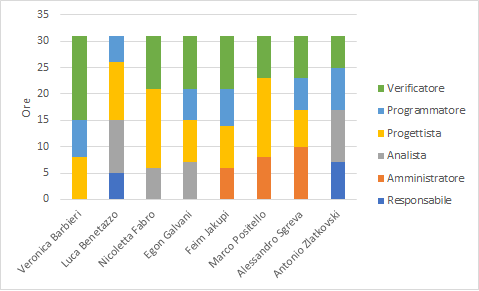
\includegraphics[width=0.7\textwidth]{./res/img/progettazioneArchitetturale_po.png}
			\caption{Suddivisione oraria del quattordicesimo incremento}
		\end{figure}
	
		\subsubsubsection{Prospetto economico}
		In base al prospetto orario, quello economico sarà il seguente: 
		\rowcolors{2}{lightRowColor}{darkRowColor}
		\begin{longtable}{
				>{\centering}p{0.25\textwidth}
				>{\centering}p{0.05\textwidth}
				>{\centering\arraybackslash}p{0.15\textwidth} }
			
			\coloredTableHead
			\textbf{\color{white}Ruolo} &
			\textbf{\color{white}Ore} &
			\textbf{\color{white}Costo in \euro{}}
			\tabularnewline
			\endhead
			
			% Contenuto della tabella
			% Ruolo & Ore & Costo \\
			Responsabile    & 3  & 90,00 \\
			Amministratore  & 4  & 80,00 \\
			Analista        & 0  & 0,00 \\
			Progettista     & 8  & 176,00 \\
			Programmatore   & 16  & 240,00 \\
			Verificatore    & 10  & 150,00 \\
			\textbf{Totale} & 41 & 736,00 \\
			
			\rowcolor{white}\caption {Prospetto dei costi per il quattordicesimo incremento}	\\
			
		\end{longtable}
		
		% Grafico
		Rappresentazione grafica della distribuzione dei ruoli:
		\begin{figure}[h]
			\centering
			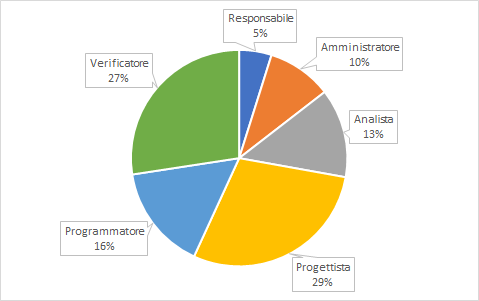
\includegraphics[width=0.7\textwidth]{./res/img/progettazioneArchitetturale_pe.png}
			\caption{Prospetto economico del quattordicesimo incremento}
		\end{figure}
	\subsubsection{15$^{\circ}$ Incremento}
		\subsubsubsection{Prospetto orario}
		Durante il quindicesimo incremento la distribuzione oraria preventivata dei ruoli di ogni componente del gruppo sarà la seguente:
		\rowcolors{2}{lightRowColor}{darkRowColor}
		\begin{longtable}{
				>{\centering}p{0.25\textwidth}
				>{\centering}p{0.05\textwidth}
				>{\centering}p{0.05\textwidth}
				>{\centering}p{0.05\textwidth}
				>{\centering}p{0.05\textwidth}
				>{\centering}p{0.05\textwidth}
				>{\centering}p{0.05\textwidth}
				>{\centering\arraybackslash}p{0.15\textwidth} }
			
			\coloredTableHead
			\textbf{\color{white}Nome} &
			\textbf{\color{white}Rp} &
			\textbf{\color{white}As} &
			\textbf{\color{white}An} &
			\textbf{\color{white}Pt} &
			\textbf{\color{white}Pr} &
			\textbf{\color{white}Vf} &
			\textbf{\color{white}Totale}
			\tabularnewline
			\endhead
			
			% Contenuto della tabella
			%    Rp & As & An & Pt & Pr & Vf & Totale \\
			\VB & 1 & -  & - & - & - & - & 1 \\
			\LB & - & -  & - & - & - & - & 0 \\
			\NF & - & -  & - & - & - & - & 0 \\
			\EG & - & -  & - & - & - & - & 0 \\
			\FJ & - & 4  & - & - & - & - & 4 \\
			\MP & 2 & -  & - & - & - & - & 2 \\
			\AS & - & -  & - & - & 1 & 2 & 3 \\
			\AZ & - & -  & - & 2 & - & - & 2 \\
			\textbf{Ore totali per ruolo} & 3 & 4 & 0 & 2 & 1 & 2 & 12 \\
			
			\rowcolor{white}\caption {Suddivisione oraria del quindicesimo incremento} \\
			
		\end{longtable}
		
		% Grafico
		\begin{figure}[H]
			\centering
			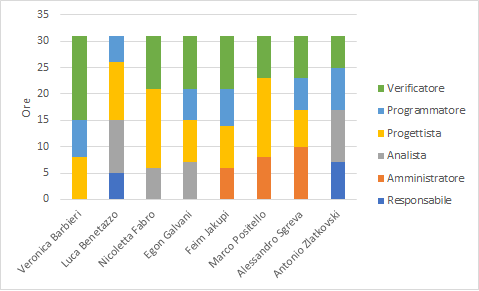
\includegraphics[width=0.7\textwidth]{./res/img/progettazioneArchitetturale_po.png}
			\caption{Suddivisione oraria del quindicesimo incremento}
		\end{figure}
	
		\subsubsubsection{Prospetto economico}
		In base al prospetto orario, quello economico sarà il seguente: 
		\rowcolors{2}{lightRowColor}{darkRowColor}
		\begin{longtable}{
				>{\centering}p{0.25\textwidth}
				>{\centering}p{0.05\textwidth}
				>{\centering\arraybackslash}p{0.15\textwidth} }
			
			\coloredTableHead
			\textbf{\color{white}Ruolo} &
			\textbf{\color{white}Ore} &
			\textbf{\color{white}Costo in \euro{}}
			\tabularnewline
			\endhead
			
			% Contenuto della tabella
			% Ruolo & Ore & Costo \\
			Responsabile    & 3  & 90,00 \\
			Amministratore  & 4  & 80,00 \\
			Analista        & 0  & 0,00 \\
			Progettista     & 2  & 44,00 \\
			Programmatore   & 1  & 15,00 \\
			Verificatore    & 2  & 30,00 \\
			\textbf{Totale} & 12 & 259,00 \\
			
			\rowcolor{white}\caption {Prospetto dei costi per il quindicesimo incremento}	\\
			
		\end{longtable}
		
		% Grafico
		Rappresentazione grafica della distribuzione dei ruoli:
		\begin{figure}[H]
			\centering
			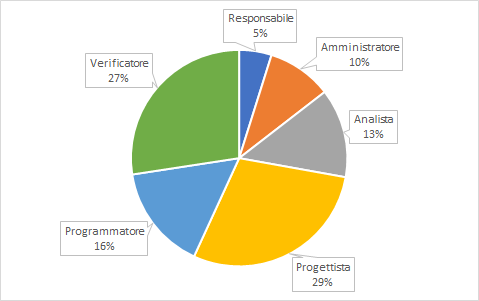
\includegraphics[width=0.7\textwidth]{./res/img/progettazioneArchitetturale_pe.png}
			\caption{Prospetto economico del quindicesimo incremento}
		\end{figure}
	\subsubsection{16$^{\circ}$ Incremento}
		\subsubsubsection{Prospetto orario}
		Durante il 16$^{\circ}$ incremento la distribuzione oraria preventivata dei ruoli di ogni componente del gruppo sarà la seguente:
		\rowcolors{2}{lightRowColor}{darkRowColor}
		\begin{longtable}{
				>{\centering}p{0.25\textwidth}
				>{\centering}p{0.05\textwidth}
				>{\centering}p{0.05\textwidth}
				>{\centering}p{0.05\textwidth}
				>{\centering}p{0.05\textwidth}
				>{\centering}p{0.05\textwidth}
				>{\centering}p{0.05\textwidth}
				>{\centering\arraybackslash}p{0.15\textwidth} }
			
			\coloredTableHead
			\textbf{\color{white}Nome} &
			\textbf{\color{white}Rp} &
			\textbf{\color{white}As} &
			\textbf{\color{white}An} &
			\textbf{\color{white}Pt} &
			\textbf{\color{white}Pr} &
			\textbf{\color{white}Vf} &
			\textbf{\color{white}Totale}
			\tabularnewline
			\endhead
			
			% Contenuto della tabella
			%    Rp & As & An & Pt & Pr & Vf & Totale \\
			\VB & - & -  & - & - & - & - & 0 \\
			\LB & - & -  & - & - & - & - & 0 \\
			\NF & - & -  & - & - & - & - & 0 \\
			\EG & - & -  & - & - & - & - & 0 \\
			\FJ & - & -  & - & - & - & - & 0 \\
			\MP & 2 & -  & - & - & - & - & 2 \\
			\AS & - & -  & - & - & 1 & 2 & 3 \\
			\AZ & - & 2  & - & 3 & - & - & 5 \\
			\textbf{Ore totali per ruolo} & 2 & 2 & 0 & 3 & 1 & 2 & 10 \\
			
			\rowcolor{white}\caption {Suddivisione oraria del 16$^{\circ}$ incremento} \\
			
		\end{longtable}
		
		% Grafico
		\begin{figure}[H]
			\centering
			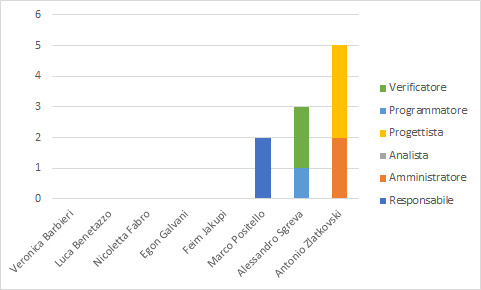
\includegraphics[width=0.7\textwidth]{./res/img/preventivi/inc16_po.png}
			\caption{Suddivisione oraria del 16$^{\circ}$ incremento}
		\end{figure}
	
		\subsubsubsection{Prospetto economico}
		In base al prospetto orario, quello economico sarà il seguente: 
		\rowcolors{2}{lightRowColor}{darkRowColor}
		\begin{longtable}{
				>{\centering}p{0.25\textwidth}
				>{\centering}p{0.05\textwidth}
				>{\centering\arraybackslash}p{0.15\textwidth} }
			
			\coloredTableHead
			\textbf{\color{white}Ruolo} &
			\textbf{\color{white}Ore} &
			\textbf{\color{white}Costo in \euro{}}
			\tabularnewline
			\endhead
			
			% Contenuto della tabella
			% Ruolo & Ore & Costo \\
			Responsabile    & 2  & 60,00 \\
			Amministratore  & 2  & 40,00 \\
			Analista        & 0  & 0,00 \\
			Progettista     & 3  & 66,00 \\
			Programmatore   & 1  & 15,00 \\
			Verificatore    & 2  & 30,00 \\
			\textbf{Totale} & 10 & 211,00 \\
			
			\rowcolor{white}\caption {Prospetto dei costi per il 16$^{\circ}$ incremento}	\\
			
		\end{longtable}
		
		% Grafico
		Rappresentazione grafica della distribuzione dei ruoli:
		\begin{figure}[H]
			\centering
			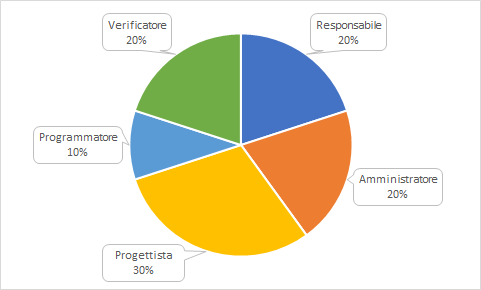
\includegraphics[width=0.7\textwidth]{./res/img/preventivi/inc16_pe.png}
			\caption{Prospetto economico del 16$^{\circ}$ incremento}
		\end{figure}
	\subsubsection{Fase complessiva}

\subsubsubsection{Prospetto orario}
Distribuzione delle ore per ciascun ruolo nel periodo di Progettazione di dettaglio e codifica:

\rowcolors{2}{lightRowColor}{darkRowColor}
\begin{longtable}{
		>{\centering}p{0.25\textwidth}
		>{\centering}p{0.05\textwidth}
		>{\centering}p{0.05\textwidth}
		>{\centering}p{0.05\textwidth}
		>{\centering}p{0.05\textwidth}
		>{\centering}p{0.05\textwidth}
		>{\centering}p{0.05\textwidth}
		>{\centering\arraybackslash}p{0.15\textwidth} }
	
	\coloredTableHead
	\textbf{\color{white}Nome} &
	\textbf{\color{white}Rp} &
	\textbf{\color{white}As} &
	\textbf{\color{white}An} &
	\textbf{\color{white}Pt} &
	\textbf{\color{white}Pr} &
	\textbf{\color{white}Vf} &
	\textbf{\color{white}Totale}
	\tabularnewline
	\endhead
	
	% Contenuto della tabella
	% Nome & Rp & As & An & Pt & Pr & Vf & Totale \\
	\VB & 7 & 4 & - & 6  & 20 & 12 & 49 \\
	\LB & - & - & - & 15 & 20 & 14 & 49 \\
	\NF & - & 8 & - & 12 & 19 & 10 & 49 \\
	\EG & 6 & - & - & 15 & 20 & 8  & 49 \\
	\FJ & 5 & 5 & - & 10 & 19 & 10 & 49 \\
	\MP & 5 & 6 & - & 8  & 15 & 15 & 49 \\
	\AS & - & - & - & 14 & 20 & 15 & 49 \\
	\AZ & - & 9 & - & 8  & 20 & 12 & 49 \\
	\textbf{Ore totali per ruolo} & 23 & 32 & - & 88 & 153 & 96 & 392 \\
	
	\rowcolor{white}\caption {Suddivisione oraria del periodo di Progettazione di dettaglio e codifica} \\
	
\end{longtable}

% Grafico
Rappresentazione grafica della suddivisione oraria:
\begin{figure}[h]
	\centering
	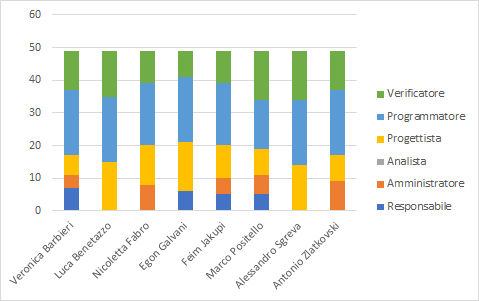
\includegraphics[width=0.7\textwidth]{./res/img/progettazioneDettaglioCodifica_po.png}
	\caption{Suddivisione oraria del periodo di Progettazione di dettaglio e codifica}
\end{figure}


\subsubsubsection{Prospetto economico}
	Totale delle ore e costo per ciascun ruolo nel periodo di Progettazione di dettaglio e codifica:

	\rowcolors{2}{lightRowColor}{darkRowColor}
	\begin{longtable}{
		>{\centering}p{0.25\textwidth}
		>{\centering}p{0.05\textwidth}
		>{\centering\arraybackslash}p{0.15\textwidth} }

		\coloredTableHead
		\textbf{\color{white}Ruolo} &
		\textbf{\color{white}Ore} &
		\textbf{\color{white}Costo in \euro{}}
		\tabularnewline
		\endhead

		% Contenuto della tabella
		% Ruolo & Ore & Costo \\
		Responsabile    & 23 & 690,00 \\
		Amministratore  & 32 & 640,00 \\
		Analista        & -  & - \\
		Progettista     & 88 & 1.936,00 \\
		Programmatore   & 153 & 2.295,00 \\
		Verificatore    & 96  & 1.440,00 \\
		\textbf{Totale} & 392 & 7.001,00 \\

		\rowcolor{white}\caption {Prospetto dei costi per il periodo di Progettazione di dettaglio e codifica} \\

	\end{longtable}

	% Grafico
	Rappresentazione grafica della distribuzione dei ruoli:
	\begin{figure}[h]
		\centering
		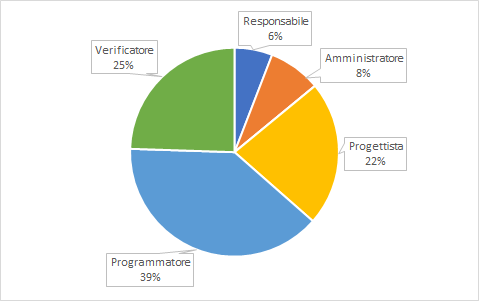
\includegraphics[width=0.7\textwidth]{./res/img/progettazioneDettaglioCodifica_pe.png}
		\caption{Suddivisione dei ruoli nel periodo di Progettazione di dettaglio e codifica}
	\end{figure}

\newpage
\subsection{Validazione e Collaudo}
	\subsubsection{17$^{\circ}$ Incremento}
		\subsubsubsection{Prospetto orario}
		Durante il 17$^{\circ}$ incremento la distribuzione oraria preventivata dei ruoli di ogni componente del gruppo sarà la seguente:
		\rowcolors{2}{lightRowColor}{darkRowColor}
		\begin{longtable}{
				>{\centering}p{0.25\textwidth}
				>{\centering}p{0.05\textwidth}
				>{\centering}p{0.05\textwidth}
				>{\centering}p{0.05\textwidth}
				>{\centering}p{0.05\textwidth}
				>{\centering}p{0.05\textwidth}
				>{\centering}p{0.05\textwidth}
				>{\centering\arraybackslash}p{0.15\textwidth} }
			
			\coloredTableHead
			\textbf{\color{white}Nome} &
			\textbf{\color{white}Rp} &
			\textbf{\color{white}As} &
			\textbf{\color{white}An} &
			\textbf{\color{white}Pt} &
			\textbf{\color{white}Pr} &
			\textbf{\color{white}Vf} &
			\textbf{\color{white}Totale}
			\tabularnewline
			\endhead
			
			% Contenuto della tabella
			%    Rp & As & An & Pt & Pr & Vf & Totale \\
			\VB & - & -  & - & 3 & - & 2 & 5 \\
			\LB & - & 3  & - & - & - & - & 3 \\
			\NF & 3 & -  & - & - & - & - & 3 \\
			\EG & - & 3  & - & - & - & 2 & 5 \\
			\FJ & 4 & -  & - & - & - & - & 4 \\
			\MP & - & -  & - & - & 3 & - & 3 \\
			\AS & - & -  & - & - & 2 & - & 2 \\
			\AZ & - & -  & - & - & - & 5 & 5 \\
			\textbf{Ore totali per ruolo} & 7 & 6 & 0 & 3 & 5 & 9 & 30 \\
			
			\rowcolor{white}\caption {Suddivisione oraria del 17$^{\circ}$ incremento} \\
			
		\end{longtable}
		
		% Grafico
		\begin{figure}[H]
			\centering
			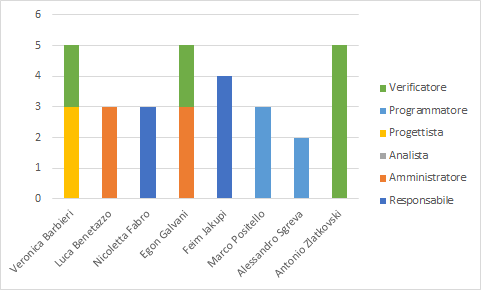
\includegraphics[width=0.7\textwidth]{./res/img/preventivi/inc17_po.png}
			\caption{Suddivisione oraria del 17$^{\circ}$ incremento}
		\end{figure}
	
		\subsubsubsection{Prospetto economico}
		In base al prospetto orario, quello economico sarà il seguente: 
		\rowcolors{2}{lightRowColor}{darkRowColor}
		\begin{longtable}{
				>{\centering}p{0.25\textwidth}
				>{\centering}p{0.05\textwidth}
				>{\centering\arraybackslash}p{0.15\textwidth} }
			
			\coloredTableHead
			\textbf{\color{white}Ruolo} &
			\textbf{\color{white}Ore} &
			\textbf{\color{white}Costo in \euro{}}
			\tabularnewline
			\endhead
			
			% Contenuto della tabella
			% Ruolo & Ore & Costo \\
			Responsabile    & 7  & 210,00 \\
			Amministratore  & 6  & 120,00 \\
			Analista        & 0  & 0,00 \\
			Progettista     & 3  & 66,00 \\
			Programmatore   & 5  & 75,00 \\
			Verificatore    & 9  & 135,00 \\
			\textbf{Totale} & 30 & 606,00 \\
			
			\rowcolor{white}\caption {Prospetto dei costi per il 17$^{\circ}$ incremento}	\\
			
		\end{longtable}
		
		% Grafico
		Rappresentazione grafica della distribuzione dei ruoli:
		\begin{figure}[H]
			\centering
			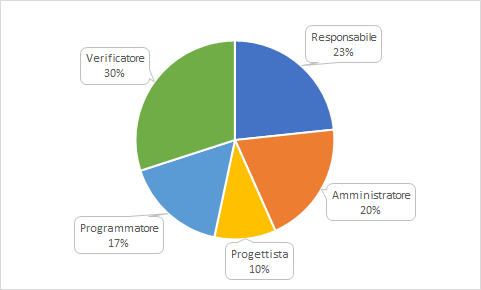
\includegraphics[width=0.7\textwidth]{./res/img/preventivi/inc17_pe.png}
			\caption{Prospetto economico del 17$^{\circ}$ incremento}
		\end{figure}
	\subsubsection{18$^{\circ}$ Incremento}

	\subsubsubsection{Consuntivo}
		\begin{longtable}{
				>{\centering}p{0.25\textwidth}
				>{\centering}p{0.08\textwidth}
				>{\centering}p{0.08\textwidth}
				>{\centering}p{0.15\textwidth}
				>{\centering\arraybackslash}p{0.15\textwidth} }

			\coloredTableHead
			\textbf{\color{white}Ruolo} &
			\textbf{\color{white}Ore} &
			\textbf{\color{white}Delta ore} &
			\textbf{\color{white}Costo in \euro{}} &
			\textbf{\color{white}Delta costo}
			\tabularnewline
			\endhead

			% Contenuto della tabella
			% Ruolo & OreEffettive & DeltaOre & Costo & DeltaCosto \\
      Responsabile    & 1  & +0 & 30,00  & +  0,00 \\
      Amministratore  & 1  & +0 & 20,00  & +  0,00 \\
      Analista        & 0  & +0 & 0,00   & +  0,00 \\
      Progettista     & 3  & +0 & 66,00  & +  0,00 \\
      Programmatore   & 10 & +0 & 150,00 & +  0,00 \\
      Verificatore    & 15 & +0 & 225,00 & +  0,00 \\
			\textbf{Totale Effettivo} & \multicolumn{2}{c}{\textbf{30}} & \multicolumn{2}{c}{\textbf{491,00}} \\
			\textbf{Delta} & \multicolumn{2}{c}{\textbf{0}} & \multicolumn{2}{c}{\textbf{+0,00}} \\

			\rowcolor{white}\caption{Consuntivo per il 18$^{\circ}$ Incremento}	\\

		\end{longtable}

	\subsubsubsection{Conclusioni}
	In questo periodo ci siamo dedicati all'implementazione della funzionalità di \texttt{init} (visualizzazione informazioni utili per iniziare ad utilizzare l'applicativo), \texttt{whoami} (visualizzazione dell'indirizzo dell'utente attualmente autenticato nel sistema) e \texttt{search} (ricerca di una funzione). Queste funzionalità richiedono solamente modifiche al modulo \textit{Etherless-cli}, e sono state rispettate il monte ore e le scadenze previste.

	\subsubsubsection{Preventivo a finire rispetto al periodo}
	La pianificazione in questo incremento è stata rispettata e il bilancio risulta essere \textbf{pari}.

	\subsubsubsection{Preventivo a finire complessivo}
	Date le considerazioni precedenti, il preventivo complessivo resta invariato.

	\subsubsection{19$^{\circ}$ Incremento}
		
	\subsubsubsection{Consuntivo}
		\begin{longtable}{
				>{\centering}p{0.25\textwidth}
				>{\centering}p{0.08\textwidth}
				>{\centering}p{0.08\textwidth}
				>{\centering}p{0.15\textwidth}
				>{\centering\arraybackslash}p{0.15\textwidth} }
			
			\coloredTableHead
			\textbf{\color{white}Ruolo} &
			\textbf{\color{white}Ore} &
			\textbf{\color{white}Delta ore} &
			\textbf{\color{white}Costo in \euro{}} &
			\textbf{\color{white}Delta costo}
			\tabularnewline
			\endhead
			
			% Contenuto della tabella
			% Ruolo & OreEffettive & DeltaOre & Costo & DeltaCosto \\
			Responsabile    & 1 & +0 &   30,00 & +  0,00 \\
			Amministratore  & 1 & +0 &   20,00 & +  0,00 \\
			Analista        & 0 & +0 &   0,00 & + 0,00 \\
			Progettista     & 2 & +0 & 44,00 & + 0,00 \\
			Programmatore   & 8 & +0 &   120,00 &  +0,00 \\
			Verificatore    & 5 & +0 & 75,00 & + 0,00 \\
			\textbf{Totale Effettivo} & \multicolumn{2}{c}{\textbf{17}} & \multicolumn{2}{c}{\textbf{289,00}} \\
			\textbf{Delta} & \multicolumn{2}{c}{\textbf{0}} & \multicolumn{2}{c}{\textbf{+0,00}} \\
			
			\rowcolor{white}\caption{Consuntivo per il 19$^{\circ}$ Incremento}	\\
			
		\end{longtable}
		
	
	\subsubsubsection{Conclusioni}
	In questo periodo il gruppo si è dedicato principalmente all'implementazione della funzionalità di visualizzazione della cronologia di esecuzione dell'utente. Poichè tale funzionalità richiede delle modifiche unicamente al modulo\ped{\textit{G}} \textit{Etherless-cli} il gruppo è riuscito a rispettare la pianificazione. 
		
	\subsubsubsection{Preventivo a finire rispetto al periodo}
	La pianificazione in questo incremento è stata rispettata e il bilancio risulta essere \textbf{pari}. 
		
	\subsubsubsection{Preventivo a finire complessivo}	
	Date le considerazioni precedenti, il preventivo complessivo resta invariato.
	\subsubsection{20$^{\circ}$ Incremento}
		
	\subsubsubsection{Consuntivo}
		\begin{longtable}{
				>{\centering}p{0.25\textwidth}
				>{\centering}p{0.08\textwidth}
				>{\centering}p{0.08\textwidth}
				>{\centering}p{0.15\textwidth}
				>{\centering\arraybackslash}p{0.15\textwidth} }
			
			\coloredTableHead
			\textbf{\color{white}Ruolo} &
			\textbf{\color{white}Ore} &
			\textbf{\color{white}Delta ore} &
			\textbf{\color{white}Costo in \euro{}} &
			\textbf{\color{white}Delta costo}
			\tabularnewline
			\endhead
			
			% Contenuto della tabella
			% Ruolo & OreEffettive & DeltaOre & Costo & DeltaCosto \\
			Responsabile    & 1 & +0 &   30,00 & +  0,00 \\
			Amministratore  & 1 & +0 &   20,00 & +  0,00 \\
			Analista        & 0 & +0 &   0,00 & + 0,00 \\
			Progettista     & 2 & +0 &  44,00 & + 0,00 \\
			Programmatore   & 9 & +4 &   105,00 &  +30,00 \\
			Verificatore    & 5 & +0 & 75,00 & + 0,00 \\
			\textbf{Totale Effettivo} & \multicolumn{2}{c}{\textbf{18}} & \multicolumn{2}{c}{\textbf{274,00}} \\
			\textbf{Delta} & \multicolumn{2}{c}{\textbf{+4}} & \multicolumn{2}{c}{\textbf{+30,00}} \\
			
			\rowcolor{white}\caption{Consuntivo per il 20$^{\circ}$ Incremento}	\\
			
		\end{longtable}
		
	
	\subsubsubsection{Conclusioni}
	In questo periodo il gruppo si è dedicato principalmente all'implementazione della funzionalità di modifica di una funzione. Pur seguendo un pattern di comunicazione tra moduli già utilizzato dal gruppo, l'implementazione della funzionalità ha richiesto più tempo di quanto preventivato. 
	
	\subsubsubsection{Preventivo a finire rispetto al periodo}
	Sono state utilizzare 4 ore di lavoro non preventivate da parte dei Programmatori; questo ha portato ad un bilancio \textbf{negativo}, con una spesa in eccesso di \textbf{30,00\euro}. 
		
	\subsubsubsection{Preventivo a finire complessivo}	
	Non essendo tale spesa eccessiva e avendo ottenuto un risparmio nei periodi precedenti, il preventivo complessivo resta invariato.
	\subsubsection{21$^{\circ}$ Incremento}
		\subsubsubsection{Prospetto orario}
		Durante il 21$^{\circ}$ incremento la distribuzione oraria preventivata dei ruoli di ogni componente del gruppo sarà la seguente:
		\rowcolors{2}{lightRowColor}{darkRowColor}
		\begin{longtable}{
				>{\centering}p{0.25\textwidth}
				>{\centering}p{0.05\textwidth}
				>{\centering}p{0.05\textwidth}
				>{\centering}p{0.05\textwidth}
				>{\centering}p{0.05\textwidth}
				>{\centering}p{0.05\textwidth}
				>{\centering}p{0.05\textwidth}
				>{\centering\arraybackslash}p{0.15\textwidth} }
			
			\coloredTableHead
			\textbf{\color{white}Nome} &
			\textbf{\color{white}Rp} &
			\textbf{\color{white}As} &
			\textbf{\color{white}An} &
			\textbf{\color{white}Pt} &
			\textbf{\color{white}Pr} &
			\textbf{\color{white}Vf} &
			\textbf{\color{white}Totale}
			\tabularnewline
			\endhead
			
			% Contenuto della tabella
			%    Rp & As & An & Pt & Pr & Vf & Totale \\
			\VB & - & -  & - & - & 2 & 5 & 7 \\
			\LB & - & -  & - & - & 4 & - & 4 \\
			\NF & - & -  & - & - & 3 & 5 & 8 \\
			\EG & - & -  & - & 2 & - & 1 & 3 \\
			\FJ & - & 3  & - & - & 2 & - & 5 \\
			\MP & 3 & -  & - & - & 1 & 5 & 9 \\
			\AS & - & -  & - & - & 1 & 6 & 7 \\
			\AZ & - & -  & - & 2 & 3 & - & 5 \\
			\textbf{Ore totali per ruolo} & 3 & 3 & 0 & 4 & 16 & 22 & 48 \\
			
			\rowcolor{white}\caption {Suddivisione oraria del 21$^{\circ}$ incremento} \\
			
		\end{longtable}
		
		% Grafico
		\begin{figure}[H]
			\centering
			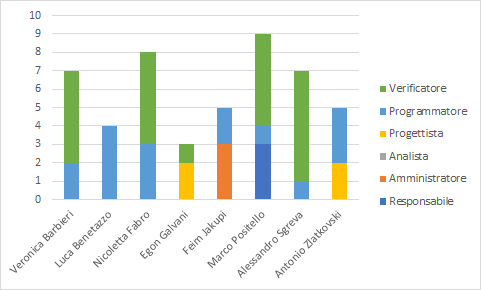
\includegraphics[width=0.7\textwidth]{./res/img/preventivi/inc21_po.png}
			\caption{Suddivisione oraria del 21$^{\circ}$ incremento}
		\end{figure}
	
		\subsubsubsection{Prospetto economico}
		In base al prospetto orario, quello economico sarà il seguente: 
		\rowcolors{2}{lightRowColor}{darkRowColor}
		\begin{longtable}{
				>{\centering}p{0.25\textwidth}
				>{\centering}p{0.05\textwidth}
				>{\centering\arraybackslash}p{0.15\textwidth} }
			
			\coloredTableHead
			\textbf{\color{white}Ruolo} &
			\textbf{\color{white}Ore} &
			\textbf{\color{white}Costo in \euro{}}
			\tabularnewline
			\endhead
			
			% Contenuto della tabella
			% Ruolo & Ore & Costo \\
			Responsabile    & 3  & 90,00 \\
			Amministratore  & 3  & 60,00 \\
			Analista        & 0  & 0,00 \\
			Progettista     & 4  & 88,00 \\
			Programmatore   & 16  & 240,00 \\
			Verificatore    & 22  & 330,00 \\
			\textbf{Totale} & 48 & 808,00 \\
			
			\rowcolor{white}\caption {Prospetto dei costi per il 21$^{\circ}$ incremento}	\\
			
		\end{longtable}
		
		% Grafico
		Rappresentazione grafica della distribuzione dei ruoli:
		\begin{figure}[H]
			\centering
			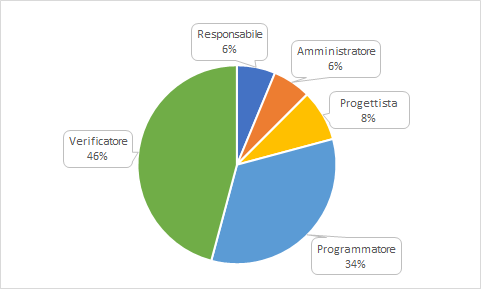
\includegraphics[width=0.7\textwidth]{./res/img/preventivi/inc21_pe.png}
			\caption{Prospetto economico del 21$^{\circ}$ incremento}
		\end{figure}
	\subsubsection{22$^{\circ}$ Incremento}
		\subsubsubsection{Prospetto orario}
		Durante il 22$^{\circ}$ Incremento la distribuzione oraria preventivata dei ruoli di ogni componente del gruppo sarà la seguente:
		\rowcolors{2}{lightRowColor}{darkRowColor}
		\begin{longtable}{
				>{\centering}p{0.25\textwidth}
				>{\centering}p{0.05\textwidth}
				>{\centering}p{0.05\textwidth}
				>{\centering}p{0.05\textwidth}
				>{\centering}p{0.05\textwidth}
				>{\centering}p{0.05\textwidth}
				>{\centering}p{0.05\textwidth}
				>{\centering\arraybackslash}p{0.15\textwidth} }
			
			\coloredTableHead
			\textbf{\color{white}Nome} &
			\textbf{\color{white}Rp} &
			\textbf{\color{white}As} &
			\textbf{\color{white}An} &
			\textbf{\color{white}Pt} &
			\textbf{\color{white}Pr} &
			\textbf{\color{white}Vf} &
			\textbf{\color{white}Totale}
			\tabularnewline
			\endhead
			
			% Contenuto della tabella
			%    Rp & As & An & Pt & Pr & Vf & Totale \\
			\VB & - & -  & - & - & - & 2 & 2 \\
			\LB & - & -  & - & - & 2 & 3 & 5 \\
			\NF & - & -  & - & - & - & 5 & 5 \\
			\EG & - & 2  & - & 1 & - & 3 & 6 \\
			\FJ & - & 2  & - & - & - & - & 2 \\
			\MP & 2 & -  & - & - & - & - & 2 \\
			\AS & 5 & -  & - & - & - & - & 5 \\
			\AZ & - & -  & - & 2 & - & 1 & 3 \\
			\textbf{Ore totali per ruolo} & 7 & 4 & 0 & 3 & 2 & 14 & 30 \\
			
			\rowcolor{white}\caption {Suddivisione oraria del 22$^{\circ}$ Incremento} \\
			
		\end{longtable}
		
		% Grafico
		\begin{figure}[H]
			\centering
			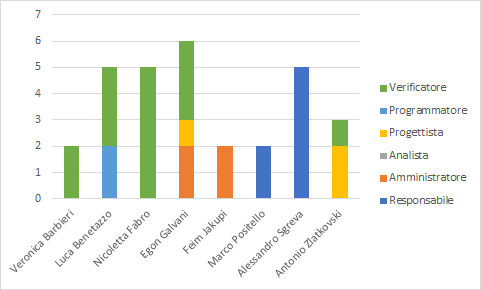
\includegraphics[width=0.7\textwidth]{./res/img/preventivi/inc22_po.png}
			\caption{Suddivisione oraria del 22$^{\circ}$ Incremento}
		\end{figure}
	
		\subsubsubsection{Prospetto economico}
		In base al prospetto orario, quello economico sarà il seguente: 
		\rowcolors{2}{lightRowColor}{darkRowColor}
		\begin{longtable}{
				>{\centering}p{0.25\textwidth}
				>{\centering}p{0.05\textwidth}
				>{\centering\arraybackslash}p{0.15\textwidth} }
			
			\coloredTableHead
			\textbf{\color{white}Ruolo} &
			\textbf{\color{white}Ore} &
			\textbf{\color{white}Costo in \euro{}}
			\tabularnewline
			\endhead
			
			% Contenuto della tabella
			% Ruolo & Ore & Costo \\
			Responsabile    & 7  & 210,00 \\
			Amministratore  & 4  & 80,00 \\
			Analista        & 0  & 0,00 \\
			Progettista     & 3  & 66,00 \\
			Programmatore   & 2  & 30,00 \\
			Verificatore    & 14  & 210,00 \\
			\textbf{Totale} & 30 & 596,00 \\
			
			\rowcolor{white}\caption {Prospetto dei costi per il 22$^{\circ}$ Incremento}	\\
			
		\end{longtable}
		
		% Grafico
		Rappresentazione grafica della distribuzione dei ruoli:
		\begin{figure}[H]
			\centering
			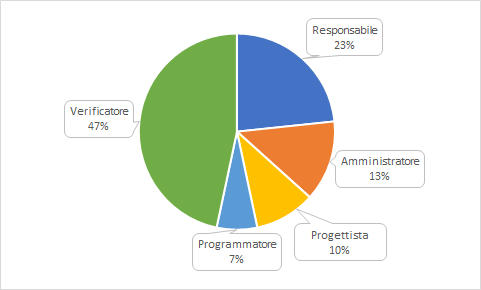
\includegraphics[width=0.7\textwidth]{./res/img/preventivi/inc22_pe.png}
			\caption{Prospetto economico del 22$^{\circ}$ Incremento}
		\end{figure}
	\subsubsection{23$^{\circ}$ Incremento}
		\subsubsubsection{Prospetto orario}
		Durante il ventitreesimo incremento la distribuzione oraria preventivata dei ruoli di ogni componente del gruppo sarà la seguente:
		\rowcolors{2}{lightRowColor}{darkRowColor}
		\begin{longtable}{
				>{\centering}p{0.25\textwidth}
				>{\centering}p{0.05\textwidth}
				>{\centering}p{0.05\textwidth}
				>{\centering}p{0.05\textwidth}
				>{\centering}p{0.05\textwidth}
				>{\centering}p{0.05\textwidth}
				>{\centering}p{0.05\textwidth}
				>{\centering\arraybackslash}p{0.15\textwidth} }
			
			\coloredTableHead
			\textbf{\color{white}Nome} &
			\textbf{\color{white}Rp} &
			\textbf{\color{white}As} &
			\textbf{\color{white}An} &
			\textbf{\color{white}Pt} &
			\textbf{\color{white}Pr} &
			\textbf{\color{white}Vf} &
			\textbf{\color{white}Totale}
			\tabularnewline
			\endhead
			
			% Contenuto della tabella
			%    Rp & As & An & Pt & Pr & Vf & Totale \\
			\VB & - & -  & - & - & - & - & 0 \\
			\LB & - & -  & - & - & - & - & 0 \\
			\NF & 1 & -  & - & - & - & - & 1 \\
			\EG & - & -  & - & 1 & - & 2 & 3 \\
			\FJ & - & 1  & - & - & 1 & - & 2 \\
			\MP & - & -  & - & - & - & - & 0 \\
			\AS & 1 & -  & - & - & - & - & 1 \\
			\AZ & - & -  & - & - & - & - & 0 \\
			\textbf{Ore totali per ruolo} & 2 & 1 & 0 & 1 & 1 & 2 & 7 \\
			
			\rowcolor{white}\caption {Suddivisione oraria del ventitreesimo incremento} \\
			
		\end{longtable}
		
		% Grafico
		\begin{figure}[h]
			\centering
			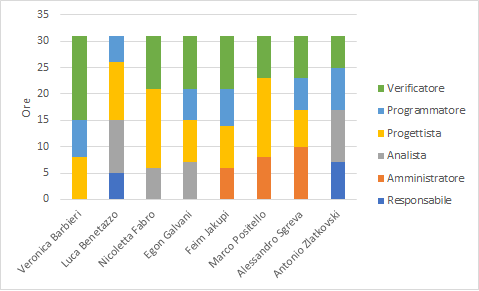
\includegraphics[width=0.7\textwidth]{./res/img/progettazioneArchitetturale_po.png}
			\caption{Suddivisione oraria del ventitreesimo incremento}
		\end{figure}
	
		\subsubsubsection{Prospetto economico}
		In base al prospetto orario, quello economico sarà il seguente: 
		\rowcolors{2}{lightRowColor}{darkRowColor}
		\begin{longtable}{
				>{\centering}p{0.25\textwidth}
				>{\centering}p{0.05\textwidth}
				>{\centering\arraybackslash}p{0.15\textwidth} }
			
			\coloredTableHead
			\textbf{\color{white}Ruolo} &
			\textbf{\color{white}Ore} &
			\textbf{\color{white}Costo in \euro{}}
			\tabularnewline
			\endhead
			
			% Contenuto della tabella
			% Ruolo & Ore & Costo \\
			Responsabile    & 2  & 60,00 \\
			Amministratore  & 1  & 20,00 \\
			Analista        & 0  & 0,00 \\
			Progettista     & 1  & 22,00 \\
			Programmatore   & 1  & 15,00 \\
			Verificatore    & 2  & 30,00 \\
			\textbf{Totale} & 7 & 147,00 \\
			
			\rowcolor{white}\caption {Prospetto dei costi per il ventitreesimo incremento}	\\
			
		\end{longtable}
		
		% Grafico
		Rappresentazione grafica della distribuzione dei ruoli:
		\begin{figure}[h]
			\centering
			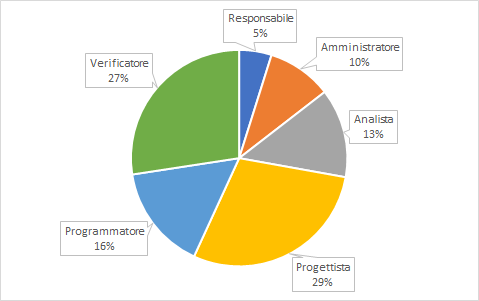
\includegraphics[width=0.7\textwidth]{./res/img/progettazioneArchitetturale_pe.png}
			\caption{Prospetto economico del ventitreesimo incremento}
		\end{figure}
	\subsection{Validazione}
    \subsubsection{Descrizione}
      Il processo di validazione stabilisce se il prodotto\ped{\textit{G}} soddisfa i requisiti richiesti, eseguendo un test completo sul sistema. Di conseguenza va eseguito in seguito al processo di verifica, il quale predispone il software per l'esecuzione di tale test. La definizione dei test da eseguire è di competenza dei Progettisti, mentre la loro esecuzione è compito dei Verificatori, che sono tenuti ad interpretarne e documentarne i risultati.
    \subsubsection{Attività}
      \subsubsubsection{Pianificazione}
      Prerequisito per l'adeguata gestione del processo di validazione è un'adeguata pianificazione. Tale pianificazione dovrebbe focalizzarsi principalmente su:
      \begin{itemize}
      	\item oggetti sottoposti a validazione;
      	\item operazioni di validazione da eseguire;
      	\item risorse, responsibilità e gestione delle scadenze legate alla pianificazione;
      	\item procedure standardizzate per l'inoltro della documentazione risultante a Proponente\ped{\textit{G}} e Committente\ped{\textit{G}}.
      \end{itemize}
      \subsubsubsection{Test di sistema [TS]}
      Già precedentemente descritti nella sezione \textsection3.5.2.2.
      \subsubsubsection{Test di accettazione [TA]}
      Nel processo di validazione viene eseguito il test di accettazione (detto anche collaudo), ovvero un test molto simile a quello di sistema, ma eseguito in collaborazione con il Committente\ped{\textit{G}}. Questo test, nello specifico, è mirato a accertare e confermare il soddisfacimento dei requisiti specificati nel capitolato\ped{\textit{G}} e analizzati nel documento \AdR{}\textit{3.0.0}. Tali test vengono rappresentati con la seguente struttura: \\
      \begin{center}
      	\textbf{TA[Importanza][Tipologia][Codice].}
      \end{center}     
      Dove:
      \begin{itemize}
      	\item{\textbf{Importanza}: indica il grado di importanza del requisito sotto test ai fini del progetto. Può assumere i valori:}
      	\begin{itemize}
      		\item{\textbf{1}: per un requisito obbligatorio;}
      		\item{\textbf{2}: per un requisito desiderabile;}
      		\item{\textbf{3}: per un requisito opzionale.}
      	\end{itemize}
      	
      	\item{\textbf{Tipologia}: rappresenta la classe a cui appartiene il requisito sotto test. Può assumere i valori:}
      	\begin{itemize}
      		\item{\textbf{F}: funzionale;}
      		\item{\textbf{P}: prestazionale;}
      		\item{\textbf{Q}: qualitativo;}
      		\item{\textbf{V}: vincolo.}
      	\end{itemize}
      	
      	\item{\textbf{Codice}: identificatore univoco del requisito sotto test}.
      \end{itemize}
    \subsubsection{Metriche}
    Un'accurata descrizione delle metriche di qualità implementate dal gruppo è presente all'interno del documento \PdQ{} \textit{3.0.0}.
    \subsubsection{Strumenti}
    Non sono attualmente stati individuati strumenti per l'attuazione dei test di sistema ed accettazione.


\subsection{Riepilogo}
	\subsubsection{Ore totali}
		\subsubsubsection{Suddivisione del lavoro}
			Distribuzione totale delle ore per ciascun ruolo comprensive delle ore di investimento e delle ore rendicontate al carico del Committente\ped{\textit{G}}.

			\rowcolors{2}{lightRowColor}{darkRowColor}
			\begin{longtable}{
				>{\centering}p{0.25\textwidth}
				>{\centering}p{0.05\textwidth}
				>{\centering}p{0.05\textwidth}
				>{\centering}p{0.05\textwidth}
				>{\centering}p{0.05\textwidth}
				>{\centering}p{0.05\textwidth}
				>{\centering}p{0.05\textwidth}
				>{\centering\arraybackslash}p{0.15\textwidth} }

				\coloredTableHead
				\textbf{\color{white}Nome} &
				\textbf{\color{white}Rp} &
				\textbf{\color{white}As} &
				\textbf{\color{white}An} &
				\textbf{\color{white}Pt} &
				\textbf{\color{white}Pr} &
				\textbf{\color{white}Vf} &
				\textbf{\color{white}Totale}
				\tabularnewline
				\endhead

				% Contenuto della tabella
				% Nome & Rp & As & An & Pt & Pr & Vf & Totale \\
				\VB & 17 & 24 & 3  & 19 & 34 & 40 & 137 \\
				\LB & 10 & 26 & 10 & 26 & 35 & 30 & 137 \\
				\NF & 5  & 28 & 6  & 37 & 26 & 35 & 137 \\
				\EG & 6  & 13 & 37 & 30 & 26 & 28 & 140 \\
				\FJ & 11 & 17 & 3  & 28 & 31 & 47 & 137 \\
				\MP & 30 & 14 & 2  & 23 & 22 & 46 & 137 \\
				\AS & 6  & 15 & 2  & 21 & 31 & 62 & 137 \\
				\AZ & 7  & 12 & 40 & 14 & 34 & 33 & 140 \\
				\textbf{Ore totali per ruolo} & 92 & 149 & 103 & 198 & 239 & 321 & 1102 \\

				\rowcolor{white}\caption {Suddivisione oraria con il totale delle ore di investimento e rendicontate}	\\

			\end{longtable}

			\newpage
			% Grafico
			Rappresentazione grafica della suddivisione oraria:
			\begin{figure}[h]
				\centering
				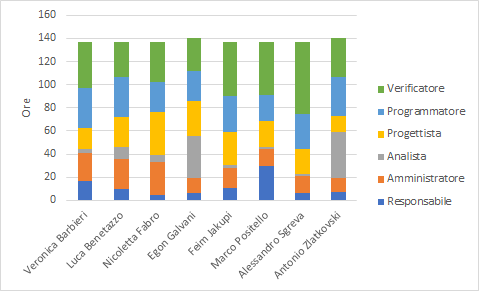
\includegraphics[width=0.7\textwidth]{./res/img/totale_po.png}
				\caption{Suddivisione oraria con il totale delle ore di investimento e rendicontate}
			\end{figure}

		\subsubsubsection{Prospetto economico}
			Totale delle ore e costo per ciascun ruolo comprensivo delle ore di investimento e delle ore rendicontate a carico del Committente\ped{\textit{G}}:

			\rowcolors{2}{lightRowColor}{darkRowColor}
			\begin{longtable}{
				>{\centering}p{0.25\textwidth}
				>{\centering}p{0.05\textwidth}
				>{\centering\arraybackslash}p{0.15\textwidth} }

				\coloredTableHead
				\textbf{\color{white}Ruolo} &
				\textbf{\color{white}Ore} &
				\textbf{\color{white}Costo in \euro{}}
				\tabularnewline
				\endhead

				% Contenuto della tabella
				% Ruolo & Ore & Costo in \\
				Responsabile    & 92   & 2.760,00 \\
				Amministratore  & 149  & 2.980,00 \\
				Analista        & 103  & 2.575,00 \\
				Progettista     & 198  & 4.356,00 \\
				Programmatore   & 239  & 3.585,00 \\
				Verificatore    & 321  & 4.815,00 \\
				\textbf{Totale} & 1102 & 21.071,00 \\

				\rowcolor{white}\caption {Prospetto dei costi totale delle ore di investimento e rendicontate per ciascun ruolo} \\

			\end{longtable}

			\newpage
			% Grafico
			Rappresentazione grafica della distribuzione dei ruoli:
			\begin{figure}[h]
				\centering
				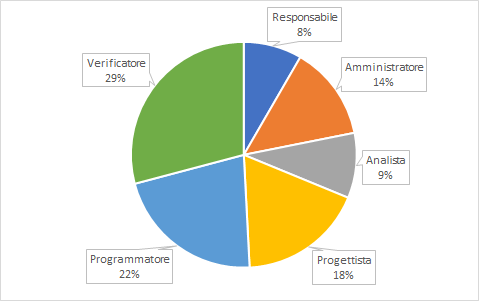
\includegraphics[width=0.7\textwidth]{./res/img/totale_pe.png}
				\caption{Suddivisione dei ruoli per il totale delle ore di investimento e rendicontate }
			\end{figure}

	\subsubsection{Ore rendicontate}
		\subsubsubsection{Suddivisione del lavoro}
			Distribuzione totale delle ore rendicontate per ciascun ruolo.

			\rowcolors{2}{lightRowColor}{darkRowColor}
			\begin{longtable}{
				>{\centering}p{0.25\textwidth}
				>{\centering}p{0.05\textwidth}
				>{\centering}p{0.05\textwidth}
				>{\centering}p{0.05\textwidth}
				>{\centering}p{0.05\textwidth}
				>{\centering}p{0.05\textwidth}
				>{\centering}p{0.05\textwidth}
				>{\centering\arraybackslash}p{0.15\textwidth} }

				\coloredTableHead
				\textbf{\color{white}Nome} &
				\textbf{\color{white}Rp} &
				\textbf{\color{white}As} &
				\textbf{\color{white}An} &
				\textbf{\color{white}Pt} &
				\textbf{\color{white}Pr} &
				\textbf{\color{white}Vf} &
				\textbf{\color{white}Totale}
				\tabularnewline
				\endhead

				% Contenuto della tabella
				% Nome & Rp & As & An & Pt & Pr & Vf & Totale \\
				\VB & 7  & 4  & -  & 19 & 34 & 38 & 102 \\
				\LB & 5  & 6  & 10 & 26 & 35 & 20 & 102 \\
				\NF & 5  & 8  & 6  & 27 & 26 & 30 & 102 \\
				\EG & 6  & 5  & 7  & 30 & 26 & 28 & 102 \\
				\FJ & 11 & 17 & -  & 18 & 31 & 25 & 102 \\
				\MP & 10 & 14 & -  & 23 & 22 & 33 & 102 \\
				\AS & 6  & 10 & -  & 21 & 31 & 34 & 102 \\
				\AZ & 7  & 9  & 10 & 14 & 34 & 28 & 102 \\
				\textbf{Ore totali per ruolo} & 57 & 73 & 33 & 178 & 239 & 236 & 816 \\

				\rowcolor{white}\caption {Suddivisione oraria con il totale delle ore rendicontate} \\

			\end{longtable}

			% Grafico
			Rappresentazione grafica della suddivisione oraria:
			\begin{figure}[h]
				\centering
				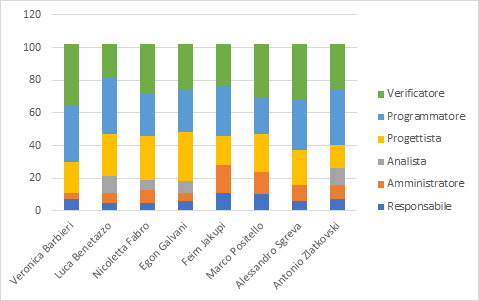
\includegraphics[width=0.7\textwidth]{./res/img/totaleRendicontate_po.png}
				\caption{Suddivisione oraria con il totale delle ore rendicontate}
			\end{figure}

		\newpage
		\subsubsubsection{Prospetto economico}
			Totale delle ore e costo per ciascun ruolo delle ore rendicontate:

			\rowcolors{2}{lightRowColor}{darkRowColor}
			\begin{longtable}{
				>{\centering}p{0.25\textwidth}
				>{\centering}p{0.05\textwidth}
				>{\centering\arraybackslash}p{0.15\textwidth} }

				\coloredTableHead
				\textbf{\color{white}Ruolo} &
				\textbf{\color{white}Ore} &
				\textbf{\color{white}Costo in \euro{}}
				\tabularnewline
				\endhead

				% Contenuto della tabella
				% Ruolo & Ore & Costo in \\
				Responsabile    & 57  & 1.710,00 \\
				Amministratore  & 73  & 1.460,00 \\
				Analista        & 33  & 825,00 \\
				Progettista     & 178 & 3.916,00 \\
				Programmatore   & 239 & 3.585,00 \\
				Verificatore    & 236 & 3.540,00 \\
				\textbf{Totale} & 816 & 15.036,00 \\

				\rowcolor{white}\caption {Prospetto dei costi totale delle ore rendicontate per ciascun ruolo} \\

			\end{longtable}

			\newpage
			% Grafico
			Rappresentazione grafica della distribuzione dei ruoli:
			\begin{figure}[h]
				\centering
				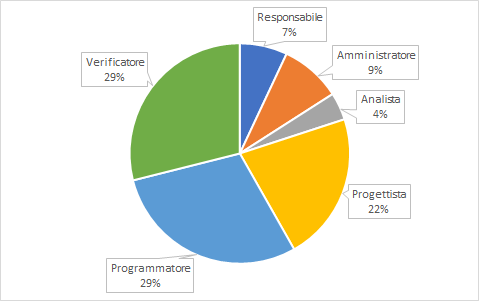
\includegraphics[width=0.7\textwidth]{./res/img/totaleRendicontate_pe.png}
				\caption{Suddivisione dei ruoli per il totale delle ore rendicontate}
			\end{figure}


\subsection{Conclusioni}
		Il costo preventivato totale per il progetto è di \textbf{\euro15.036,00}.
